\cleardoublepage

\chapter{Influence of sleep inertia on DRF}
\label{res:inertia}

% \includepdf[pages=-, pagecommand={\thispagestyle{plain}}]{Articles/Vallat_Sleep_Inertia_NI.pdf}

\section{Brain networks dynamics during sleep inertia}
\label{res:inertia:inertia}

\bigskip

\textbf{{\large Reduced default mode network connectivity and anti-correlation in the minutes following awakening from N2 and N3 sleep: an EEG-fMRI study}}

\hfill Under review at \emph{Neuroimage}

\bigskip

Raphael Vallat\textsuperscript{1} (PhD candidate), David Meunier\textsuperscript{1} (PhD), Alain Nicolas\textsuperscript{1,2} (M.D, PhD), Perrine Ruby\textsuperscript{1} (PhD)

\textsuperscript{1} Lyon Neuroscience Research Center, Brain Dynamics and Cognition team, INSERM UMRS 1028, CNRS UMR 5292, Université Claude Bernard Lyon 1, Université de Lyon, Lyon, France

\textsuperscript{2} Unité Michel Jouvet, Centre Hospitalier Le Vinatier, 95 boulevard Pinel, Lyon, France

\subsection*{Summary}
\label{res:inertia:inertia:summary}

The transition from sleep to wake is characterized by reduced vigilance, sleepiness and impaired performances, a state often referred to as sleep inertia. Even though the behavioral aspects of sleep inertia are well documented, its cerebral correlates remain poorly understood. Using combined EEG-fMRI in 55 participants, we examined the brain functional connectivity during sleep inertia before and after a 45 minutes mid-afternoon nap. Resting-state scans were acquired before the nap, 5 min and 25 min after awakening from N2 sleep (n=14) or N3 sleep (n=20). Results showed that sleep inertia is associated with an intrusion of sleep specific functional connectivity into wakefulness, which severity is dependent of the prior sleep duration and sleep depth. Awakening in N3 sleep induced the most robust changes and was characterized by a loss of brain functional segregation between task-negative and task-positive networks.

% \subsection*{Abbreviations}
% \label{res:inertia:inertia:abbr}
% rCBF: regional cerebral blood flow, fMRI: functional magnetic resonance imaging, DMN: default mode network, DAN: dorsal attention network, FP: frontoparietal control network, SM: sensorimotor network, NREM: non rapid eye movement sleep, DST: descending subtraction task

\subsection*{Introduction}
\label{res:inertia:inertia:intro}

Sleep inertia is defined as a transient period occurring just after awakening from sleep, and characterized by reduced vigilance, sleepiness and impaired cognitive and physical performances \citep{tassi_sleep_2000, trotti_waking_2016}. As Trotti clearly pointed out in the title of her article \q{waking up is the hardest thing I do all day}, sleep inertia is also usually experienced as unpleasant. Although its duration is not consensual and varies depending on the outcome measure used, it is generally admitted that most of the behavioral effects of sleep inertia dissipate progressively in the first 30 minutes post awakening. Severity of sleep inertia has been positively associated to several factors such as prior sleep deprivation, awakening near the circadian trough of body temperature, awakening in slow-wave sleep (see \citet{tassi_sleep_2000} for a review) and some sleep disorders. Excessive sleep inertia, sometimes referred to as sleep drunkenness, is indeed a core feature of idiopathic hypersomnia and a component of delayed sleep phase disorder and NREM arousal parasomnias \citep{trotti_waking_2016}.

A better understanding of sleep inertia is needed for the development of new strategies to reduce its detrimental effects on cognitive and physical performances, in pathological or physiological context alike. Sleep inertia may indeed have critical consequences in emergency situations when individuals are required to make vital decisions or actions immediately upon awakening (e.g. medical staff, firemen, pilots, military). In the general population, sleep inertia represents the main limiting factor to the numerous beneficial effects of daytime napping \citep{faraut_napping:_2016}.

The behavioral aspects of sleep inertia are well documented, but only a limited amount of studies investigated its cerebral correlates until now. Using EEG, some studies have found a persistence of slow wave activity in the minutes following awakening, specifically in posterior areas, a phenomenon which has been suggested to represent the electrophysiological signature of sleep inertia \citep{ogilvie_falling_1992, ferrara_electroencephalographic_2006, marzano_recalling_2011, gorgoni_eeg_2015}. Using PET, \citet{balkin_process_2002} reported that the brain areas whose regional cerebral blood flow (rCBF) was increasing between 5 to 20 min post awakening (p-a) were primarily anterior heteromodal areas (e.g. lateral prefrontal cortices, and anterior insula). They also reported shifts in the relative levels of rCBF between pairs of brain regions (orbitofrontal cortex and ventromedial caudate nucleus, dorsolateral prefrontal cortex and mesencephalic reticular formation) between 5 and 20 min post awakening, leading them to propose that recovery from sleep inertia could hinge on a resumption of normal levels of both rCBF and functional connectivity between brain areas. The latter hypothesis has been tested in two recent resting-state functional magnetic resonance imaging (fMRI) studies which investigated the variations in brain connectivity between pre-sleep wakefulness, nocturnal sleep (without previous sleep deprivation) and post-sleep wakefulness \citep{wu_variations_2012, tsai_local_2014}. Using paired comparisons between pre- and post-sleep wakefulness, they found a decreased connectivity within the sensory-motor (SM) network at awakening but no alterations in the default mode network (DMN). This altered connectivity within the sensory-motor network is coherent with the poor motor performances observed at awakening but does not explain the impairments observed in other domains (e.g. cognitive tasks such as mental calculation, \citealp{tassi_sleep_2000, trotti_waking_2016}).

Some modifications of the DMN connectivity could be expected at awakening since several neuroimaging studies showed consistent alterations of the DMN connectivity during sleep, fatigue and/or falling asleep (see \citet{picchioni_sleep_2013} for a review). During N1 and N2 sleep, several teams found a decrease in the anti-correlation between the default mode network on one hand and task-positive networks on the other (i.e. dorsal attention and executive control networks). This decreased anti-correlation has also been observed during wake after total or partial sleep deprivation, in addition with robust alterations across the whole brain functional connectome \citep{samann_increased_2010, de_havas_sleep_2012, yeo_functional_2015, kaufmann_brain_2015, tushaus_resisting_2017}. Finally, during deep sleep (N3 or slow-wave sleep), several studies reported a strong disruption of DMN connectivity and anti-correlation \citep{horovitz_decoupling_2009, larson-prior_modulation_2011, samann_development_2011}, as well as an absence of frontoparietal connectivity \citep{spoormaker_frontoparietal_2012}). Altogether, these results argue in favor of a progressive loss of functional segregation of brain networks from sleep onset to deep sleep, which might explain why the behavioral impairments at awakening are the most acute when individuals are awakened in N3 sleep and lead to the hypothesis that awakening from N3 sleep should be associated with DMN functional connectivity disruption.

In order to improve our understanding of sleep inertia, we designed a study with several novelties compared to previous ones. First, we used a combined EEG-fMRI method to acquire resting state scans before sleep, 5 min after awakening and 25 min after awakening in 55 healthy young participants. This design enabled us to investigate the dynamic of functional connectivity in several brain networks during the first half hour following awakening. Second, participants were partially sleep deprived on the night before and awakened from a 45 min mid-afternoon nap, in the deepest possible sleep stage (N3 sleep). Both sleep deprivation and awakening in N3 sleep have been associated with increased sleep inertia \citep{tassi_sleep_2000}. In addition with being ecological (short nights compensated by a daytime nap being common in young adults \citep{faraut_napping:_2016}, this paradigm allowed us to study sleep inertia in its most intensified form. Finally, each resting-state scan was paired with a mental calculation task in order to measure the behavioral effects of sleep inertia.

Using such a design we aimed at characterizing the brain functional connectivity just after awakening from deep sleep (N3) and its modulation in the first half hour after awakening. A total of 55 participants were included, of which 20 were awakened in N3 sleep and 14 in N2 sleep, allowing us to describe and compare the functional connectivity during sleep inertia following awakening from these two distinct sleep stages.

We expected a decrease in performances 5 min p-a compared to pre-sleep and 25 min p-a. We hypothesized that (1) the functional connectivity 5 min after awakening would share some features with the one of the sleep stage that was ongoing before awakening, i.e. we notably expected to observe a decrease in DMN connectivity and anti-correlation after awakening from N2 or N3 sleep (2) a decreased connectivity within the SM network (3) a positive correlation between the severity of performance impairments and functional connectivity disruption at awakening on the one hand and sleep depth before awakening on the other hand.

\subsection*{Methods}
\label{res:inertia:inertia:methods}

\subsubsection*{Participants}
Fifty-five participants (28 males, mean age = 22.55, standard deviation = 2.41, range = 19–29) were included in the study. The subjects were informed of the study through an announcement sent to several mailing lists of Lyon University. Participants were selected if they reported having a regular sleep-wake schedule, no difficulty to fall asleep, being occasional or frequent nappers and having preferentially already done an MRI brain scan in the past few years. They had no history of neurological and psychiatric disorders, and had no sleep disturbances. They provided written informed consent according to the Declaration of Helsinki and received monetary compensation for their participation. The study was approved by the local ethics committee (CCPPRB, Centre Leon Berard, Lyon, France).

\subsubsection*{Experimental design}
The experimental design is presented in Fig 1.

\begin{figure}[htb]
	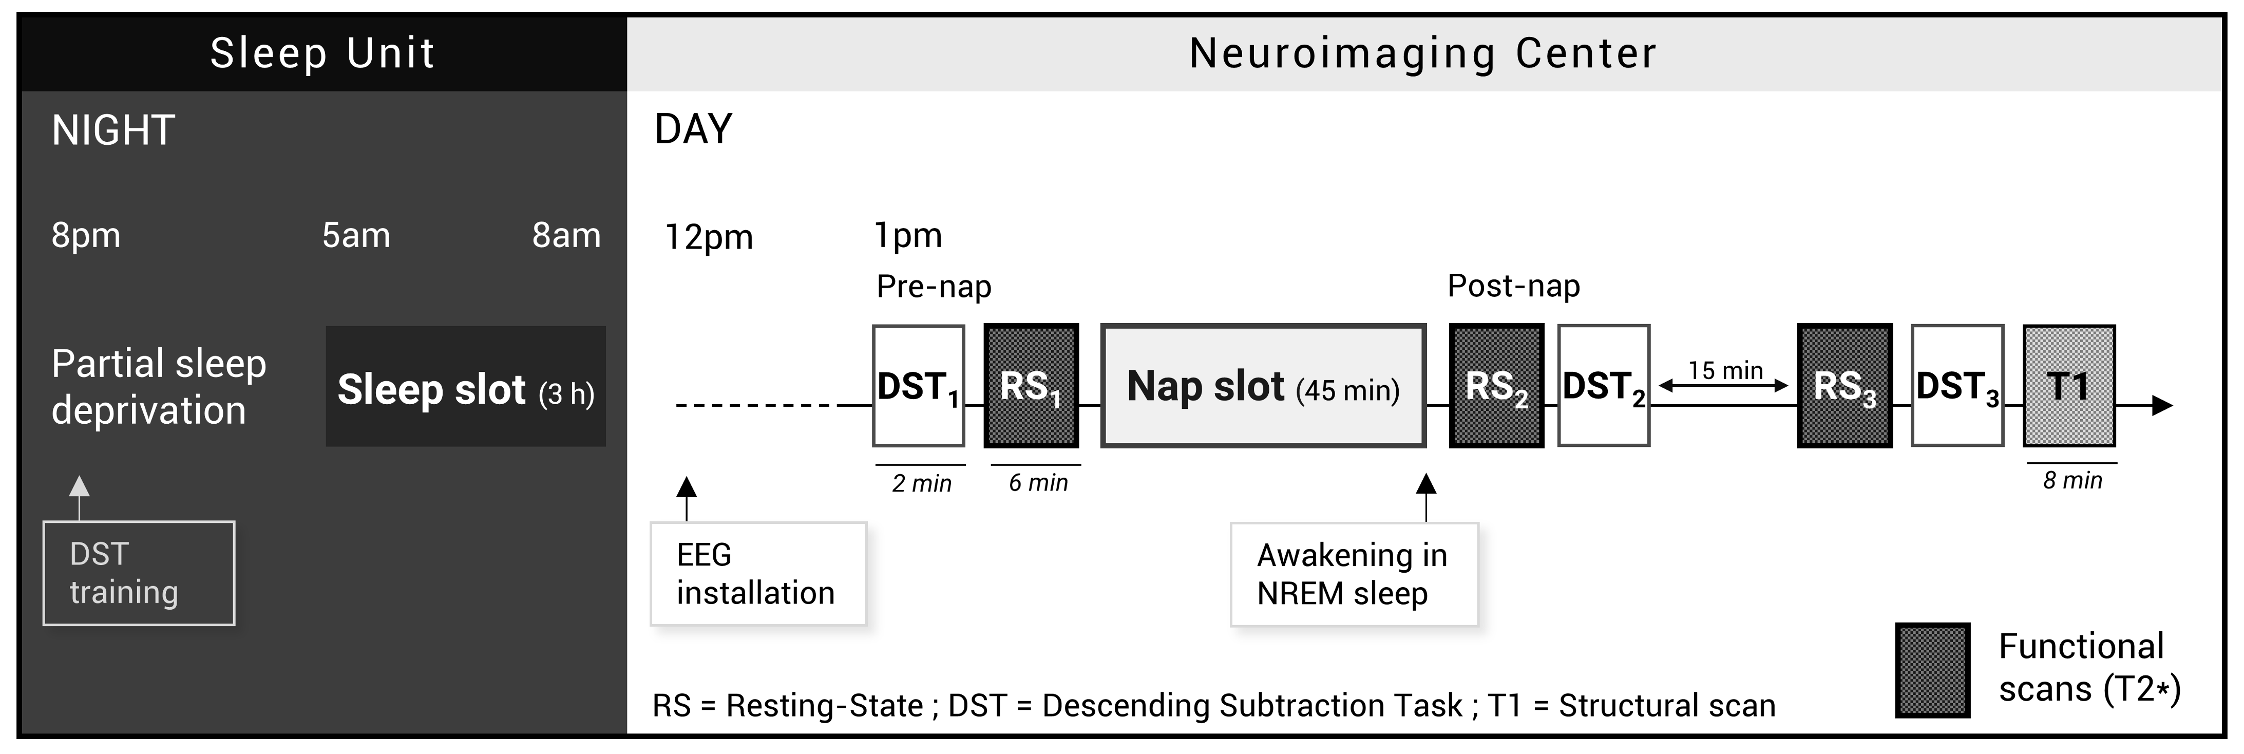
\includegraphics[width=\textwidth]{Fig/Results/Inertia/Inertia/Fig1_Protocol.png}
	\caption*{\textbf{Fig 1. Experimental design}}
\end{figure}

\emph{Evening and night}. Participants arrived in the sleep unit of the hospital Le Vinatier (Lyon, France) at 8 pm on the evening prior to the experimental day. From 8 pm to 10 pm, they underwent several personality and cognitive tests (results will be presented elsewhere) administered by R.V. They were then instructed to stay awake until 5 am (the possible activities were reading, making puzzles and watching movies), at which point they were allowed to sleep for 3 hours until 8 am in a bed in the sleep unit. Energy drinks or physical activity were prohibited during the partial sleep deprivation, and nurses regularly checked that the subject did not fall asleep. The monitoring of body movements through wrist actigraphy (Actigraph, Pensacola, USA) during the whole night made it possible to check a posteriori that the subject did not fall asleep before 5 am. In the morning, participants were offered breakfast and a shower and then occupied themselves (reading or internet) under the experimenters’ supervision until the MRI session.

\emph{Day}. After lunch at 11.30 am, participants were conducted to the neuroimaging center (CERMEP). During the first half hour, experimenters installed on the participant’s head a MRI compatible EEG cap (EASYCAP®). Participants were then installed in the MRI scanner at about 1.20 pm (1.17 pm ± 13 min). They read a 5 min cartoon during the calibration of the eye-tracking camera, and then did the DST for 2 minutes. The first resting-state scan was then acquired, with the instructions to remain awake and look at a central fixation cross on the screen. At the end of the scan, participants were informed that they could sleep (at 1.39 pm ± 14 min in average) during the next 45 min. At the end of the nap slot, participants were awakened, if they were sleeping, by calling their first name and the 2nd resting state scan was acquired in the following minutes. At the end of the scan, the 2nd DST was performed. During the following 10 minutes, questions about sleep in the scanner and about the cartoon were asked to the subjects (results will be reported elsewhere). Then the 3rd resting state scan and DST were performed (about 25 min after awakening). Finally, an 8-min T1 anatomical scan was acquired. When they got out of the MRI, participants completed a questionnaire about their thoughts during the three resting state scans.

\subsubsection*{Behavioral tasks}
To evaluate the time course of the dissipation of sleep inertia we used the descending subtraction task (DST) that has been previously used to evidence performances decrement and normalization in the first 30 min post awakening \citep{dinges_assessing_1985, evans_recovery_1975, stampi_ultrashort_1990}. Subjects were presented with a three-digit number. They were instructed to subtract 9, saying the operation and the result aloud, and then continue by subtracting 8 from the remainder, then 7, and so on until they had to subtract 1. At this point they were to start the cycle of descending subtractions again. They had to do the task for two minutes and were instructed to be as fast and accurate as possible. As this task has a substantial practice effect over the first trials \citep{dinges_assessing_1985}, participants were trained the night before the fMRI session (they performed the task six times during the evening in the sleep unit).

The outcome measures from the DST are: 1) the total number of responses, which is an index of the speed of information processing, 2) the percentage of mistakes, which is a marker of accuracy, 3) the percentage of correct responses (relative to pre-nap performances), which is a marker of both speed and accuracy \citep{dinges_assessing_1985}. Since several studies reported that speed is generally more impaired than accuracy during sleep inertia \citep{trotti_waking_2016}, we expected a significant decrement of post-nap performances especially for the total number and percentage of responses.

\subsubsection*{EEG data collection}
Polysomnography data were recorded using a 15 channels MR-compatible cap designed for sleep studies i.e. with a layout designed according to American Academy of Sleep Medicine Guidelines 2007 (EasyCap, Brain Products GmbH, Gilching, Germany). It comprised 9 EEG electrodes placed according to the international standard 10/20 system (O1, O2, C3, C4, F3, F4, M1, M2, Cz, FCz was used as reference and AFz as ground), 2 EOG electrodes, 3 EMG electrodes, and an electrocardiogram electrode placed on the back of the participant. The sampling rate was 5000 Hz and an analog band-pass filter was set to 0.01 – 250 Hz. To score sleep online during the fMRI session, a real-time pulse-artefact correction was applied using the BrainVision Recorder (Version 1.2) and BrainVision RecView (Version 1.4) softwares (Brain Products).

To ensure that participants were not closing their eyes during the resting state scans, eye movements were monitored during the experiment using an EyeLink 1000 fMRI eye tracking system (SR Research Ontario, Canada). Eye position was calibrated at the beginning of the experiment and monitored throughout.

\subsubsection*{MRI data collection}
MRI scans were obtained from a MAGNETOM Prisma 3.0 T scanner (Siemens Healthcare, Erlangen, Germany) at the Primage neuroimaging platform (CERMEP). Structural MRI were acquired with a T1-weighted (0.9-mm isotropic resolution) MPRAGE sequence and functional MRI data with a T2*-weighted 2D gradient echo planar imaging sequence (EPI) with 180 volumes (TR/TE: 2000/ 25 ms; flip angle: 80°; voxel size: 2.68 × 2.68 × 3 mm; slices: 40, duration: 6 minutes). Functional and anatomical scans were performed using a 20-channel head coil. The coil was foam-padded to improve subject comfort and restrict head motion.

\subsubsection*{EEG analysis}
Artifacts related to gradient switching and cardiac pulse (cardio-ballistic artifact) were removed using standard routines available in BrainVision Analyzer version 2.0 software (Brain Products). Polysomnographic data were downsampled to 1000 Hz and band-pass filtered between 0.5 and 25 Hz. Offline sleep stage scoring was performed using EEG epochs of 30 seconds following standard AASM rules (Iber, 2007; Silber et al., 2007) visualized using SLEEP software \citep{combrisson_sleep:_2017}. S1 Fig shows the hypnogram during the nap slot for one subject who reached N3 sleep.

\subsubsection*{fMRI analysis}
Preprocessing and quality check were performed using standard routine in SPM12 software (Wellcome Department of Imaging Neuroscience). Preprocessing included functional realignment, slice-time correction, coregistration to structural scan, spatial normalization and spatial smoothing using a 6 mm full-width at half-maximum isotropic Gaussian kernel filter. Individual T1 images were segmented into gray matter, white matter and cerebrospinal fluid tissue maps. Functional and structural images were then normalized to MNI152 space (Montreal Neurological Institute). Functional images underwent artifact and motion regression in the Artifact Detection Toolbox (\fnurl{ART}{https://www.nitrc.org/projects/artifact_detect/}) using the following criteria to define outliers: global signal intensity changes greater than 9 standard deviations and movement exceeding 2 mm. SPM motions parameters and outliers were subsequently included as covariates in connectivity analyses.

Resting-state networks and their main regions of interests (ROIs) were defined from a brain parcellation atlas implemented in the \fnurl{CONN Toolbox}{http://www.nitrc.org/projects/conn} version 17f \citep{whitfield-gabrieli_conn:_2012}. This atlas was obtained using an independent component analysis (ICA) on 467 subjects from the Human Connectome Project. Subcortical ROIs (hippocampus, thalamus, and amygdala) were defined from the Harvard-Oxford maximum likelihood subcortical atlas. Spatial maps of the ROIs used in further connectivity analyses for each network of interest are displayed in S2 Fig.

Connectivity analysis were performed using the CONN toolbox version 17f. First, we performed a denoising step including a regression of the 6 motion correction parameters and their corresponding first-order temporal derivatives, as well as a component-based strategy (aCompCor, \citealp{behzadi_component_2007}) to identify and remove physiological confounds that are unlikely to be related to neural activity. The resulting BOLD time series were band-pass filtered (0.008 – 0.09 Hz) to further reduce noise and increase sensitivity \citep{weissenbacher_correlations_2009}. Then, intra- and inter-network connectivity were calculated for each subject by extracting the mean BOLD time series of each ROI of a given network and by correlating them with the average BOLD time series of every other ROI from this network or of the other networks included in the analysis. The mean network connectivity was then computed as the mean of all pair-wise Fischer-transformed correlation coefficient within a network and compared within subjects between conditions and between subjects. In addition with the previously described ROI-to-ROI analysis, we performed seed-to-voxel analysis on the posterior cingulate cortex (PCC), one core region of the DMN which demonstrates notable disruption during NREM sleep (\citealp{picchioni_sleep_2013}; center of mass in MNI coordinates: 1, -61, 38).

\subsubsection*{Statistics}
For the descending subtraction task, between-group comparisons were achieved using a mixed two-way repeated measures ANOVA with a group factor (two levels: N2 sleep and N3 sleep, see results section) and a time factor (within subject factor with three levels: Pre-sleep, 5 min p-a, 25 min p-a). Post hoc analyses (t-tests) were used in case of significance. ROI-to-ROI connectivity analysis were conducted using two-sided t-tests corrected for multiple comparisons using the false discovery rate (FDR, p<.05). Seed-based connectivity analysis were performed using a cluster-defining voxel-wise height threshold of p<.01 (uncorrected, two-sided) and a whole-brain family-wise error (FWE) corrected extent threshold of p<.05.

\subsection*{Results}
\label{res:inertia:inertia:results}

\subsubsection*{Sleep parameters}
Despise the sleep deprivation, 20 out of 55 participants did not reach or maintain NREM sleep during the 45-min nap slot in the scanner. This result was not a surprise given the discomfort and stress inherent to the MR environment \citep{duyn_eeg-fmri_2012}. One subject out of the 35 remaining was discarded because of a technical failure during data acquisition, leading thus to a total of 34 participants included in the final analysis. We further divided these participants as a function of the sleep stages they were in before awakening. Twenty participants were awakened in N3 sleep (N3 group) and 14 participants were awakened in N2 sleep (N2 group). This allowed us to compare the functional connectivity during sleep inertia after awakening from both N2 and N3 sleep. Between-group comparisons were performed both for the functional connectivity and the behavioral data. Means of the main sleep parameters in the two groups are presented in Table 1. Importantly, there was no group difference in the latency between the awakening and the first and second post-awakening resting-state scan, respectively. Note that as expected, the sleep deprivation did succeed to maximize sleep inertia at awakening. Indeed a few participants experienced very difficult awakenings marked by a short period of panic, claustrophobia and blast of hot air, often accompanied by strong neurovegetative responses (tachycardia, hyperventilation, sudation).

\begin{table}[htb]
    \caption*{\textbf{Table 1. Sleep parameters (Mean ± SD) of the subjects in the N3 (n=20) and N2 (n=14) groups.} TST = Total Sleep Time, SE = Sleep Efficiency, Wake (W), N1, N2 and N3 = Total duration of each sleep stage in minutes. LAS1 = latency (min) between the awakening and the start of the first post-awakening resting-state scan. LAS2 = latency (min) between the awakening and the start of the second post-awakening resting-state scan.}
    \begin{tabularx}{\textwidth}{XXXXXXXXX}
    \toprule
    Group  & TST        & SE (\%)       & W         & N1         & N2         & N3          & LAS1      & LAS2 			\\ \midrule
    N2     & 38.2 ± 7.1 & 87.4 ± 9.6    & 9.1 ± 4.0 & 14.2 ± 7.6 & 21.6 ± 6.2 & 2.9 ± 4.4   & 3.7 ± 1.9 & 23.8 ± 3.7 	\\
    N3     & 37.3 ± 5.0 & 87.5 ± 7.4    & 9.2 ± 4.2 & 9.0 ± 5.7  & 17.7 ± 4.9 & 11.0 ± 4.6  & 4.8 ± 3.9 & 24.4 ± 4.2 	\\
    T-test & .68        & .99           & .95       & .03        & .05        & <.001       & .34       & .63 			\\ \bottomrule
    \end{tabularx}%
\end{table}

\subsubsection*{Descending subtraction task}
Performance at the DST during the fMRI session are presented in Fig 2. As expected, we observed a significant main effect of time [F(2, 32)=4.0, p=.02] in the total number of responses. The total number of response was lower at 5 min post-awakening as compared to 25 min post-awakening (p=.008 ; Fig 2A). There was a tendency for a reduced total number of responses at 5 min compared to pre-sleep (p=.07). No group effect or interaction were found for the total number of responses. This decrease in calculation speed at 5 min post-awakening was not associated with a significant increase in the percentage of mistakes (Fig 2B). This result is consistent with the generally held view that speed is more impaired than accuracy during sleep inertia (Trotti, 2016). However, there was a significant interaction between time and group factors [F(2,32)=3.60, p=.03]. Post-hoc tests revealed that the N2 group had a higher percentage of mistakes at 5 min post-awakening compared to the N3 group (p<.001). Finally, regarding the percentage of correct responses, which is a marker of both speed and accuracy, we also found a significant main effect of time [F(2, 32)=3.13, p=.05]. The number of correct responses was lower at 5 min post-awakening than at 25 min post-awakening (p=.01), but not significantly different before the nap as compared to 5 min after awakening (p=.17; Fig 2C). As for the total number of responses, no group effect or interaction was found for the percentage of correct responses.

\begin{figure}[htbp]
	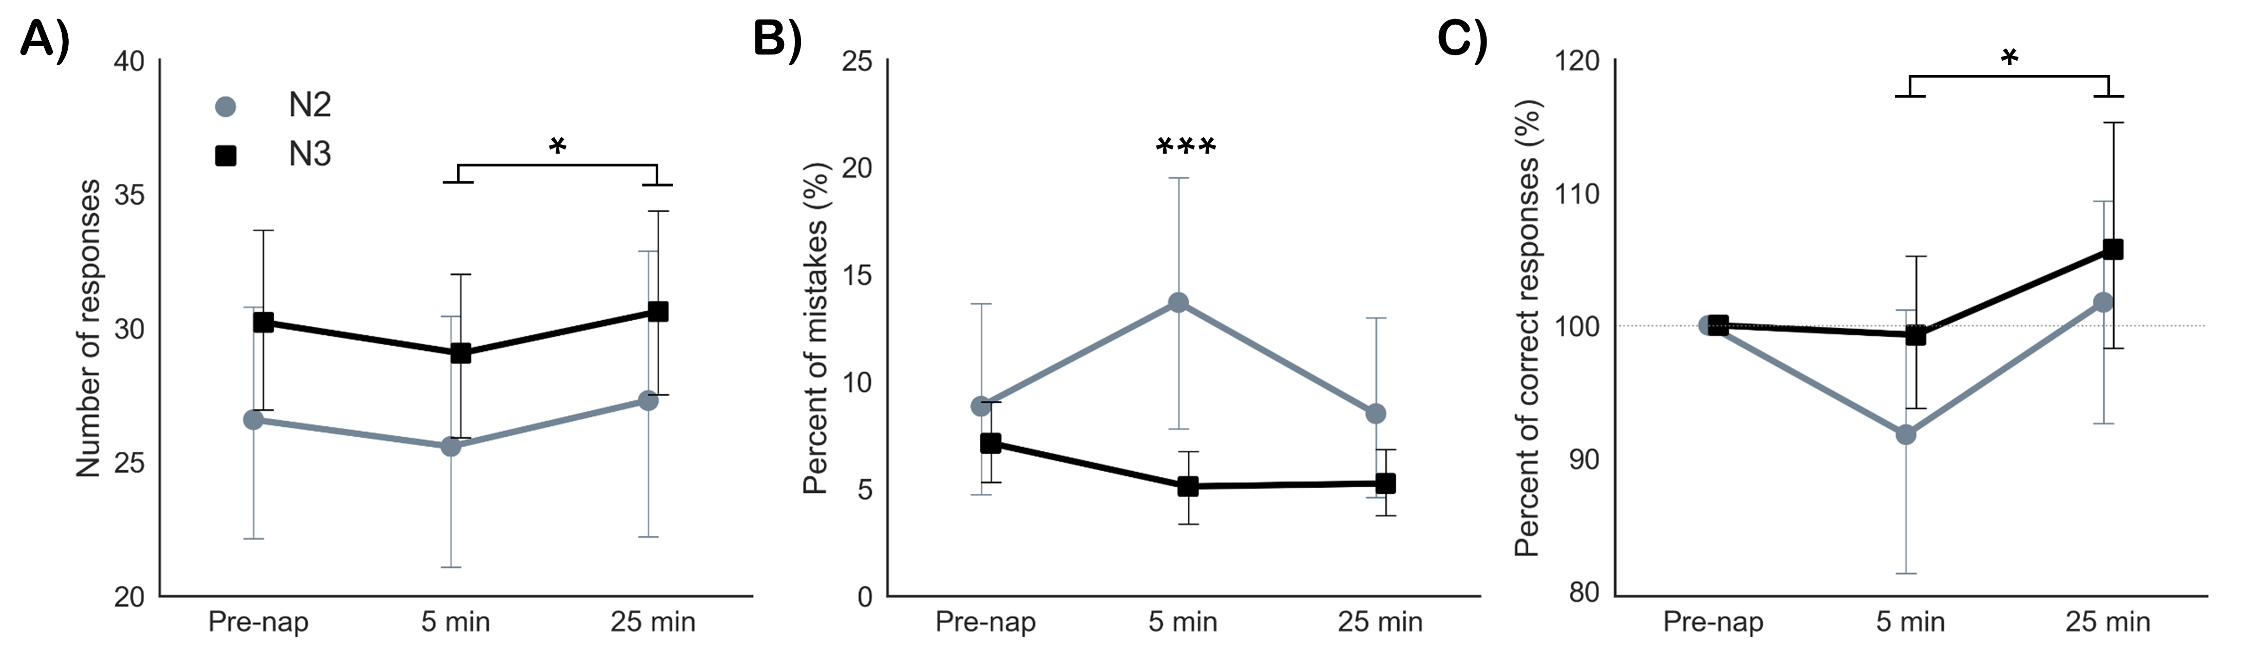
\includegraphics[width=\textwidth]{Fig/Results/Inertia/Inertia/Fig2_DST.png}
	\caption*{\textbf{Fig 2. Performances of the Descending Subtraction Task.} Blue gray lines, N2 group (n=14), black lines, N3 group (n=20). (A) Total number of responses (index of speed). (B) Percentage of mistakes (marker of accuracy). (C) Percentage of correct responses relative to pre-nap performances (marker of both speed and accuracy). Error bars represent 95\% confidence intervals. * p<.05, *** p<.001}
\end{figure}

\subsubsection*{Functional connectivity alterations following awakening from N3 sleep}
The brain functional connectivity at 5 min after awakening from N3 sleep showed important alterations. ROI-to-ROI analysis demonstrated a disrupted pattern of connectivity between several brain networks at 5 min p-a compared to pre-nap and 25 min p-a. Fig 3A illustrates the connectivity between several network, notably the DMN, DAN, fronto-parietal executive network (FP), sensori-motor (SM), salience and visual networks, in the pre-nap and 25 min p-a conditions as compared to the 5 min p-a condition. Fig 3B shows mean pairwise connectivity within and between networks. One of the most significant result was the large decrease of the anti-correlation (i.e. increased connectivity between networks that are normally anti-correlated) at 5 min p-a between the DMN and several other networks, namely the DAN, the SM, and the salience networks (Fig 3A and 3B, right). Interestingly, we observed alterations in the between-networks functional connectivity, whereas the mean within-network functional connectivity within each of these networks was not reduced at 5 min p-a compared to the two other conditions (Fig 3B, left). Seed-based analysis confirmed the disruption of the anti-correlation between the DMN (seed in the PCC) and SM network at 5 min p-a compared to pre-sleep and 25 min p-a (Fig 3C and S1 Table). In addition, there was a reduced connectivity at 5 min p-a compared to pre-sleep between the PCC and the inferior temporal gyrus, a region considered to be a part of the extended DMN and known for its role in memory and mental simulations \citep{christoff_mind-wandering_2016}.

\begin{figure}[!htbp]
	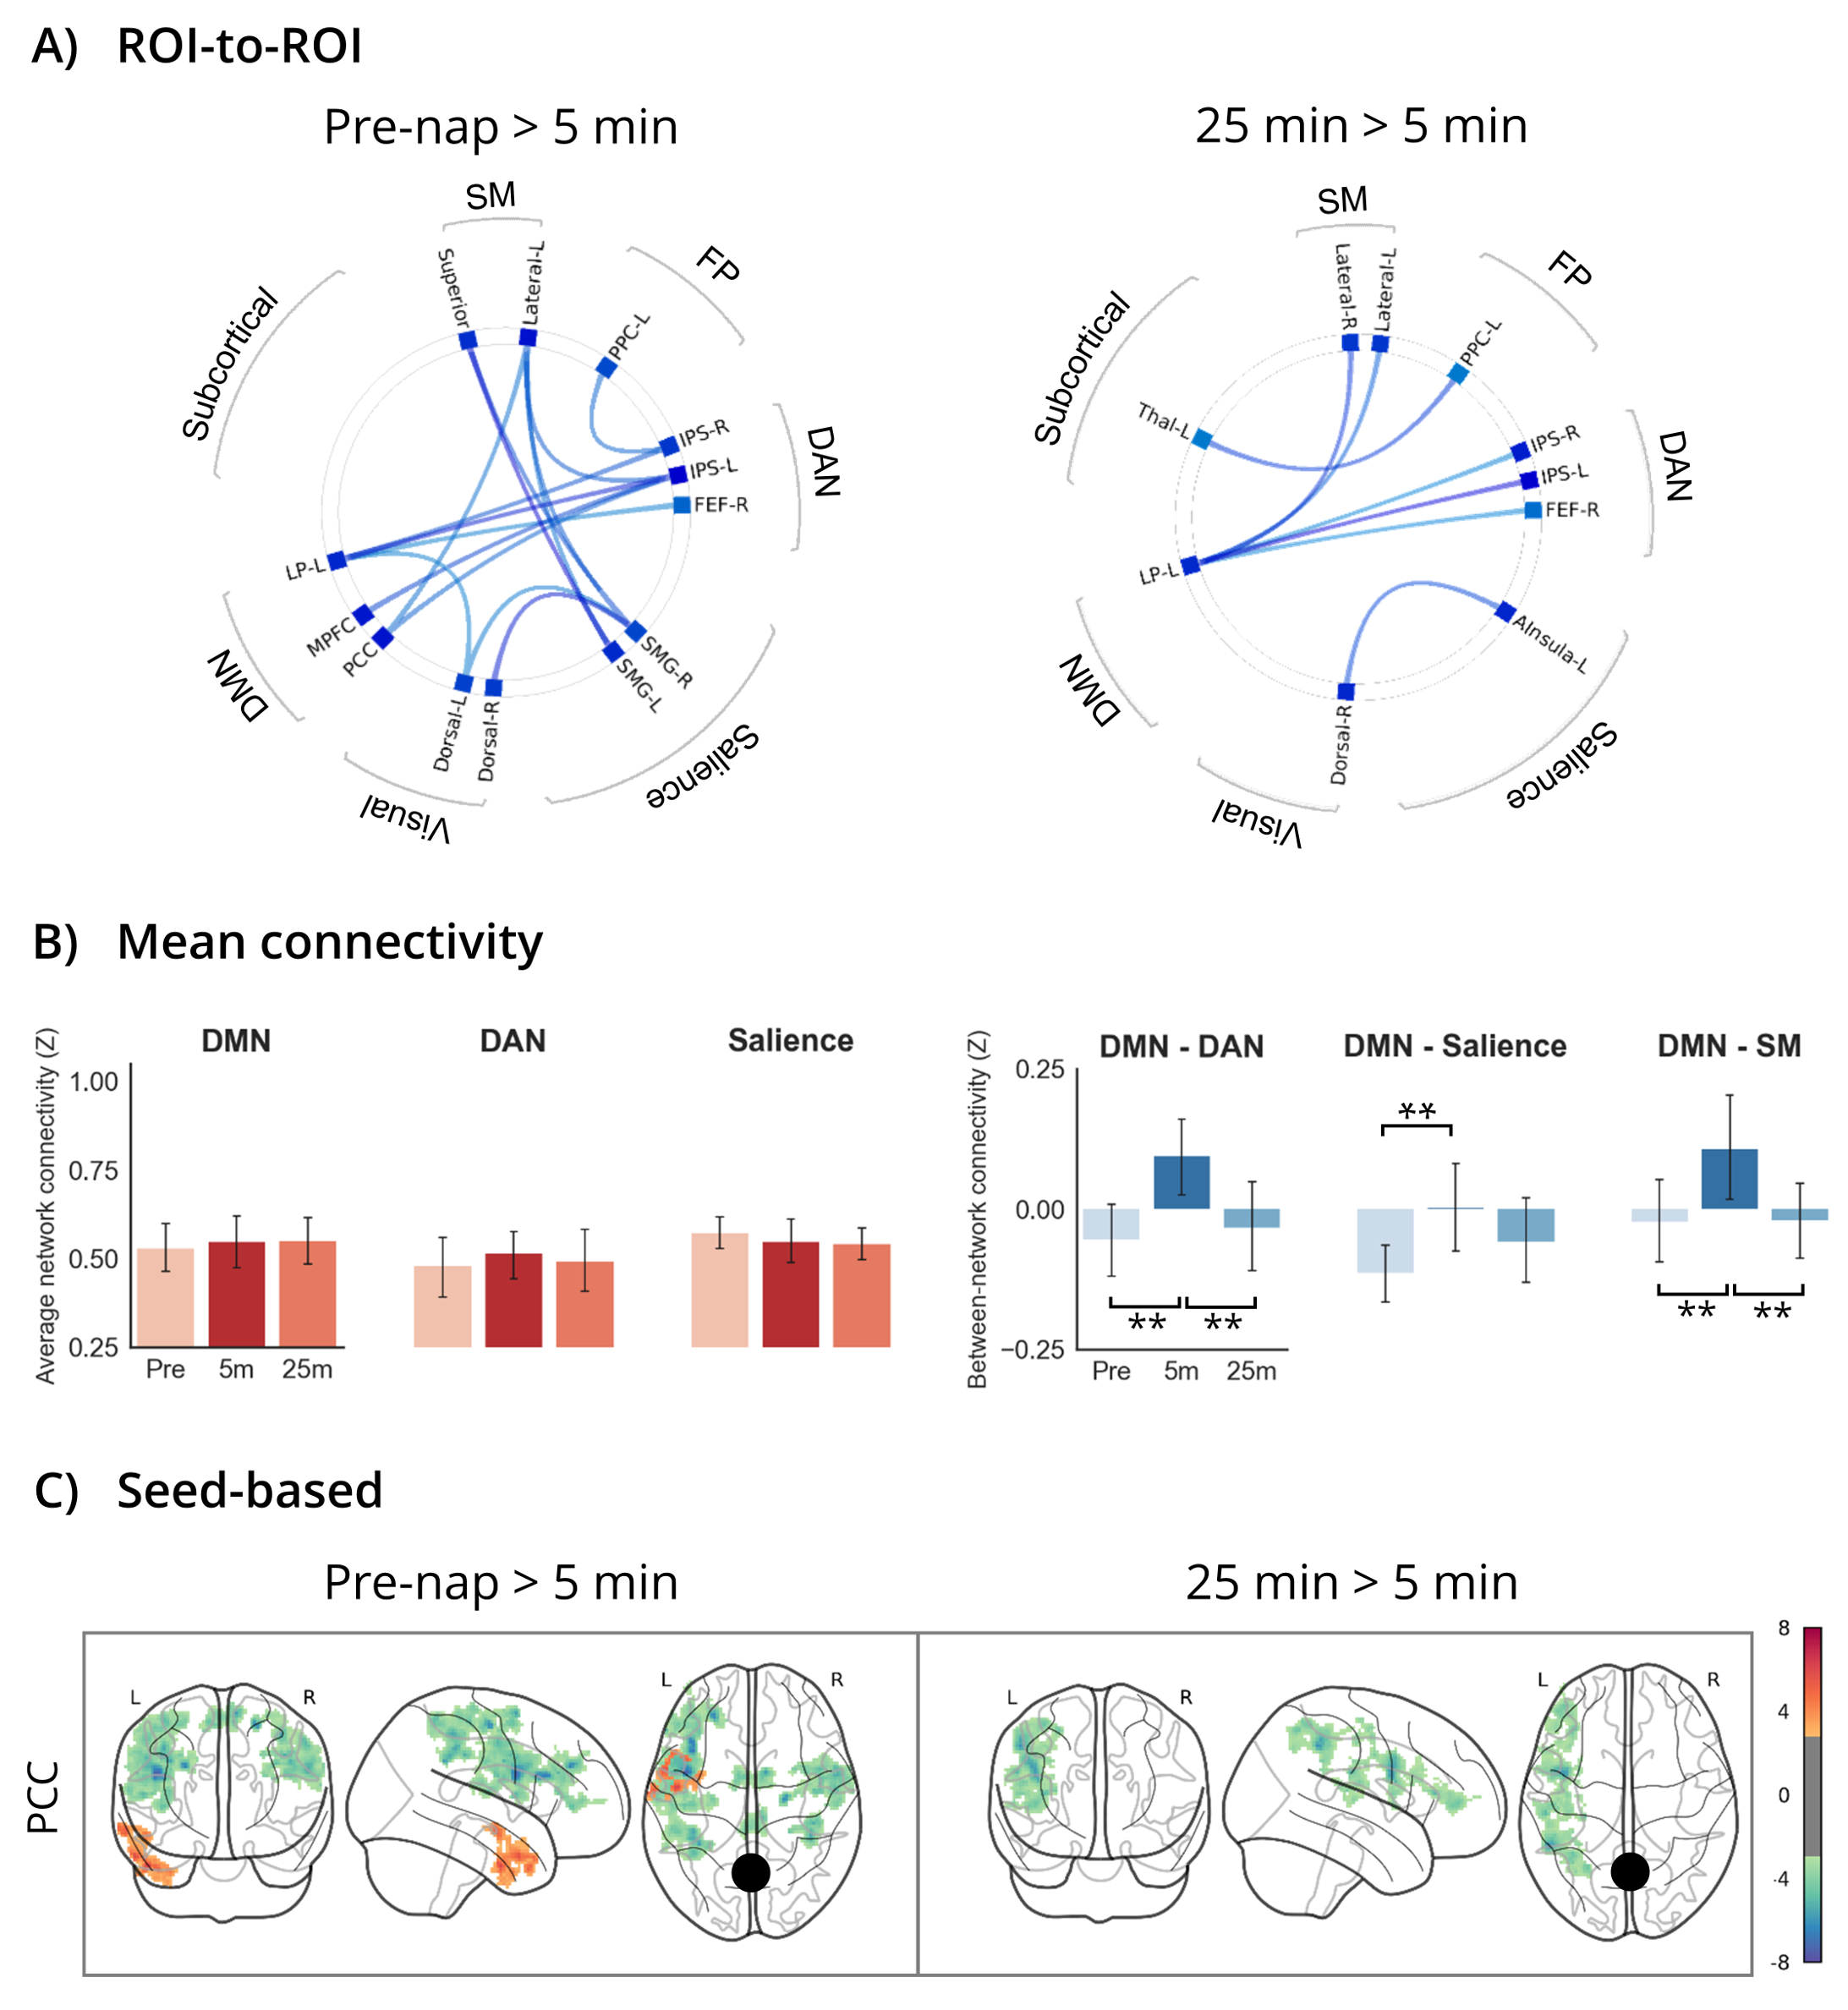
\includegraphics[width=\textwidth]{Fig/Results/Inertia/Inertia/Fig3_N3.png}
	\caption*{\textbf{Fig 3. Functional connectivity disruption after awakening from N3 sleep (n=20)}. (A) ROI-to-ROI results for the two contrasts (left, Pre-nap minus 5 min p-a; right, 25 min p-a minus 5 min p-a). Blue connections indicate regions with significantly increased pairwise connectivity (two-sided paired t-test, p<.05 FDR-corrected) at 5 min p-a compared to the pre-nap condition (left) and compared to the 25 min p-a condition (right). (B) Mean pairwise connectivity within (left, red bars) and between (right, blue bars) networks. Stars denote significant post-hoc comparisons (t-tests, ** p<.01). (C) Seed-based connectivity results for the two contrasts (left, Pre-nap minus 5 min p-a; right, 25 min p-a minus 5 min p-a). Seed region is the posterior cingulate cortex (PCC), one core region of the DMN which demonstrates notable disruption during NREM sleep (center of mass in MNI coordinates: 1, -61, 38). Statistical parametric maps are reported using an uncorrected two-sided cluster-defining voxel-wise height threshold of p<.01 and a whole-brain FWE-corrected extent threshold of p<.05. Yellow-red colors indicate increased connectivity at pre-nap and/or 25 min p-a compared to the 5 min p-a scan. Green-blue colors indicate increased connectivity at 5 min p-a compared to the two other scans.}
\end{figure}

\subsubsection*{Functional connectivity alterations following awakening from N3 sleep}
Awakening from N2 sleep was also associated with some alterations in the brain connectivity. As compared to pre-sleep, the functional connectivity at 5 min p-a was reduced between the SM and two regions of the FP network, the SM and the right hippocampus and between the ventral and dorsal part of the visual network. By contrast, the connectivity at 5 min p-a was increased between two regions of the DMN and the hippocampus and between the salience and SM networks (Fig 4A). As compared to 25 min p-a, the functional connectivity at 5 min p-a was reduced within the DAN, within the ventral and dorsal part of the visual network, and between the SM and FP networks. By contrast, connectivity was increased between the visual and salience networks (Fig 4A). The mean connectivity within and between networks was not significantly altered at 5 min p-a after an awakening in N2 sleep (Fig 4B). In accordance with these results, seed-based analysis showed an increased connectivity at 5 min-pa compared to pre-sleep between the PCC and several regions including the hippocampus and part of the SM network (Fig 4C and S2 Table). PCC connectivity was not significantly different at 25 min p-a compared to both pre-sleep and 5 min p-a.

\begin{figure}[!htbp]
	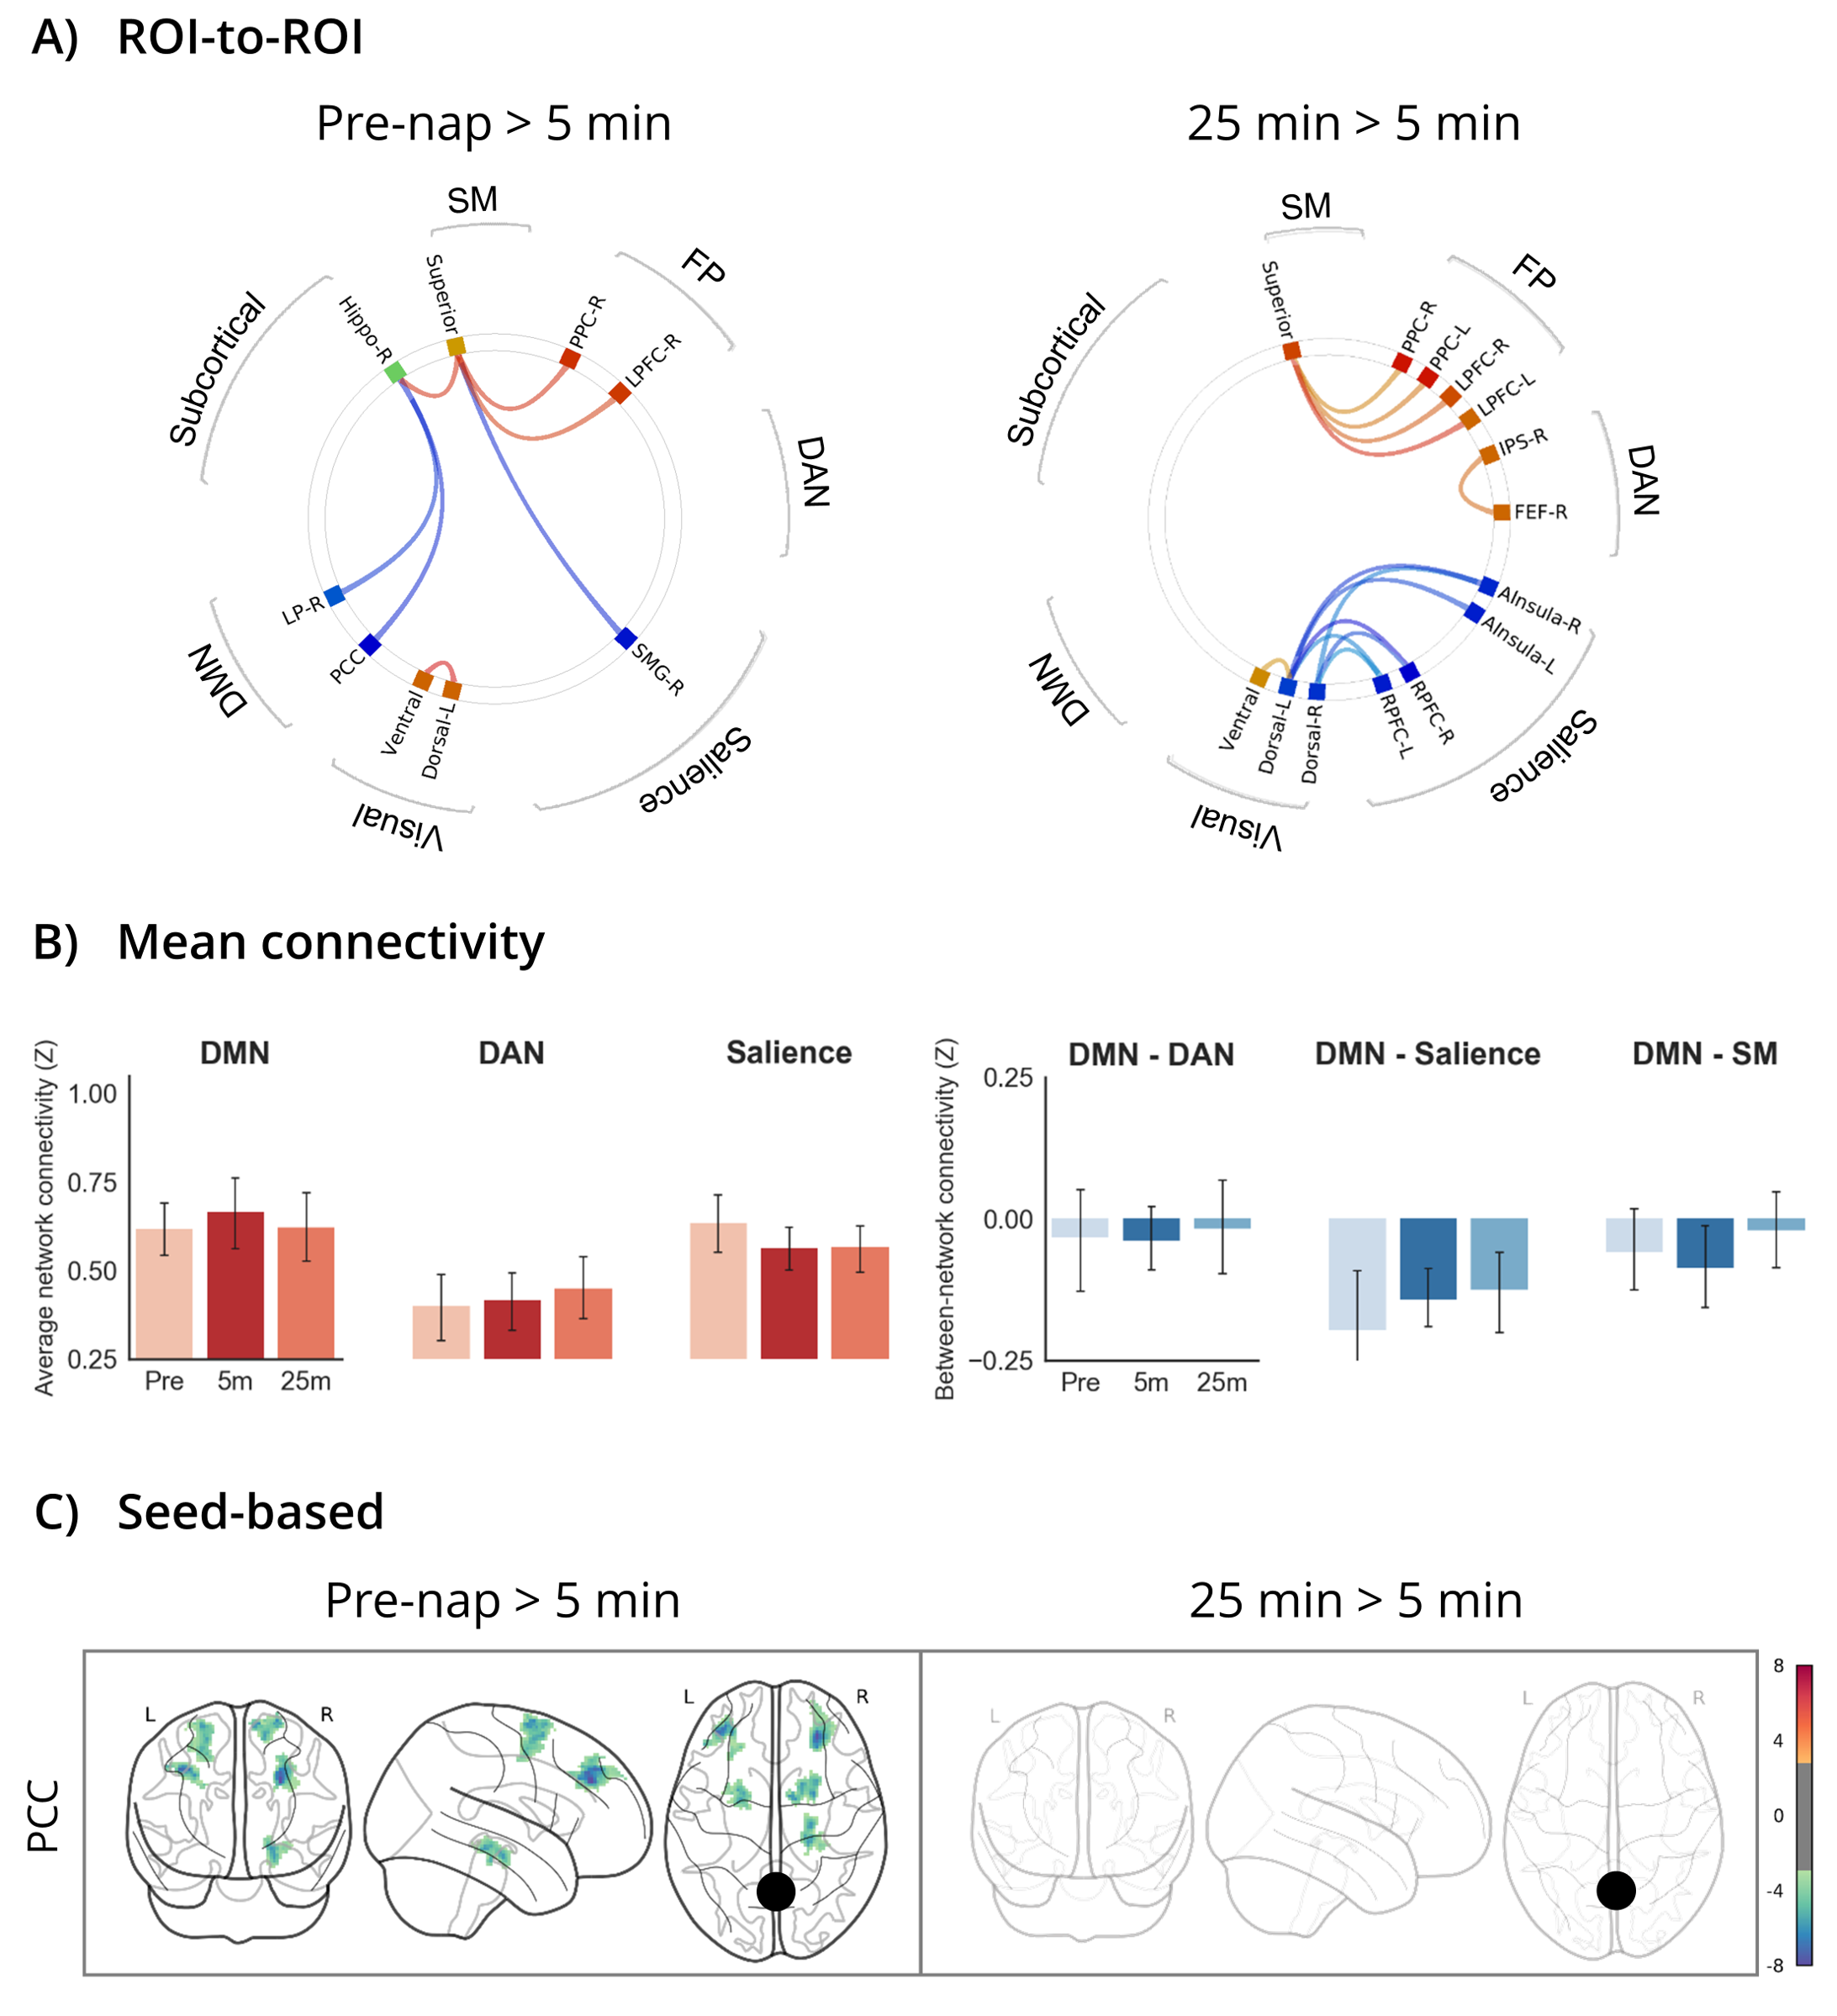
\includegraphics[width=\textwidth]{Fig/Results/Inertia/Inertia/Fig4_N2.png}
	\caption*{\textbf{Fig 4. Functional connectivity disruption after awakening from N2 sleep (n=14)}. (A) ROI-to-ROI results for the two contrasts (left, Pre-nap minus 5 min p-a; right, 25 min p-a minus 5 min p-a). Connections indicate regions with significantly increased (blue lines) or decreased (red lines) pairwise connectivity at 5 min p-a compared to the pre-nap and 25 min p-a scans, respectively (two-sided paired t-test, p<.05 FDR-corrected). (B) Mean pairwise connectivity within (left, red bars) and between (right, blue bars) networks. (C) Seed-based connectivity results for the two contrasts (left, Pre-nap minus 5 min p-a; right, 25 min p-a minus 5 min p-a). Seed region is the posterior cingulate cortex (PCC), one core region of the DMN which demonstrates notable disruption during NREM sleep (center of mass in MNI coordinates: 1, -61, 38). Statistical parametric maps are reported using an uncorrected two-sided cluster-defining voxel-wise height threshold of p<.01 and a whole-brain FWE-corrected extent threshold of p<.05. Yellow-red colors indicate increased connectivity at pre-nap and/or 25 min p-a compared to the 5 min p-a scan. Green-blue colors indicate increased connectivity at 5 min p-a compared to the two other scans.}
\end{figure}

\subsubsection*{Comparison of the functional connectivity alterations following N2 and N3 sleep awakenings}
To further investigate the relationship between functional connectivity alterations and the sleep stage before awakening, we compared the brain connectivity between the N2 and the N3 groups. First, we looked at ROI-to-ROI differences at each resting-state scan (Fig 5A). Interestingly, during the pre-nap scan, the connectivity between the FP network and two regions, the lateral parietal (part of the DMN) and hippocampus, was decreased in the N3 group. At 5 min p-a, participants awakened in N3 sleep had a significantly increased connectivity between the DMN and DAN and between the SM and three networks (DMN, FP, Visual). There was no group difference at 25 min p-a. Next, at 5 min p-a, there was a tendency for a reduced mean DMN connectivity (p=.07) and increased DAN connectivity (p=.08) in the N3 group (Fig 5B, left). Third, the anti-correlations between the DMN and the attentional network and the DMN and the sensori-motor network were significantly decreased in the N3 group (Fig 5B, right, Fig 5D and S3 Table). Finally, we found a significant negative correlation between the mean DMN connectivity at 5 min p-a and the duration of N2/N3 sleep during the nap (Spearman r = -.43, p = .01, Fig 5C). This latter results shows that functional alterations within the DMN are associated with the prior sleep duration.

\begin{figure}[!htbp]
	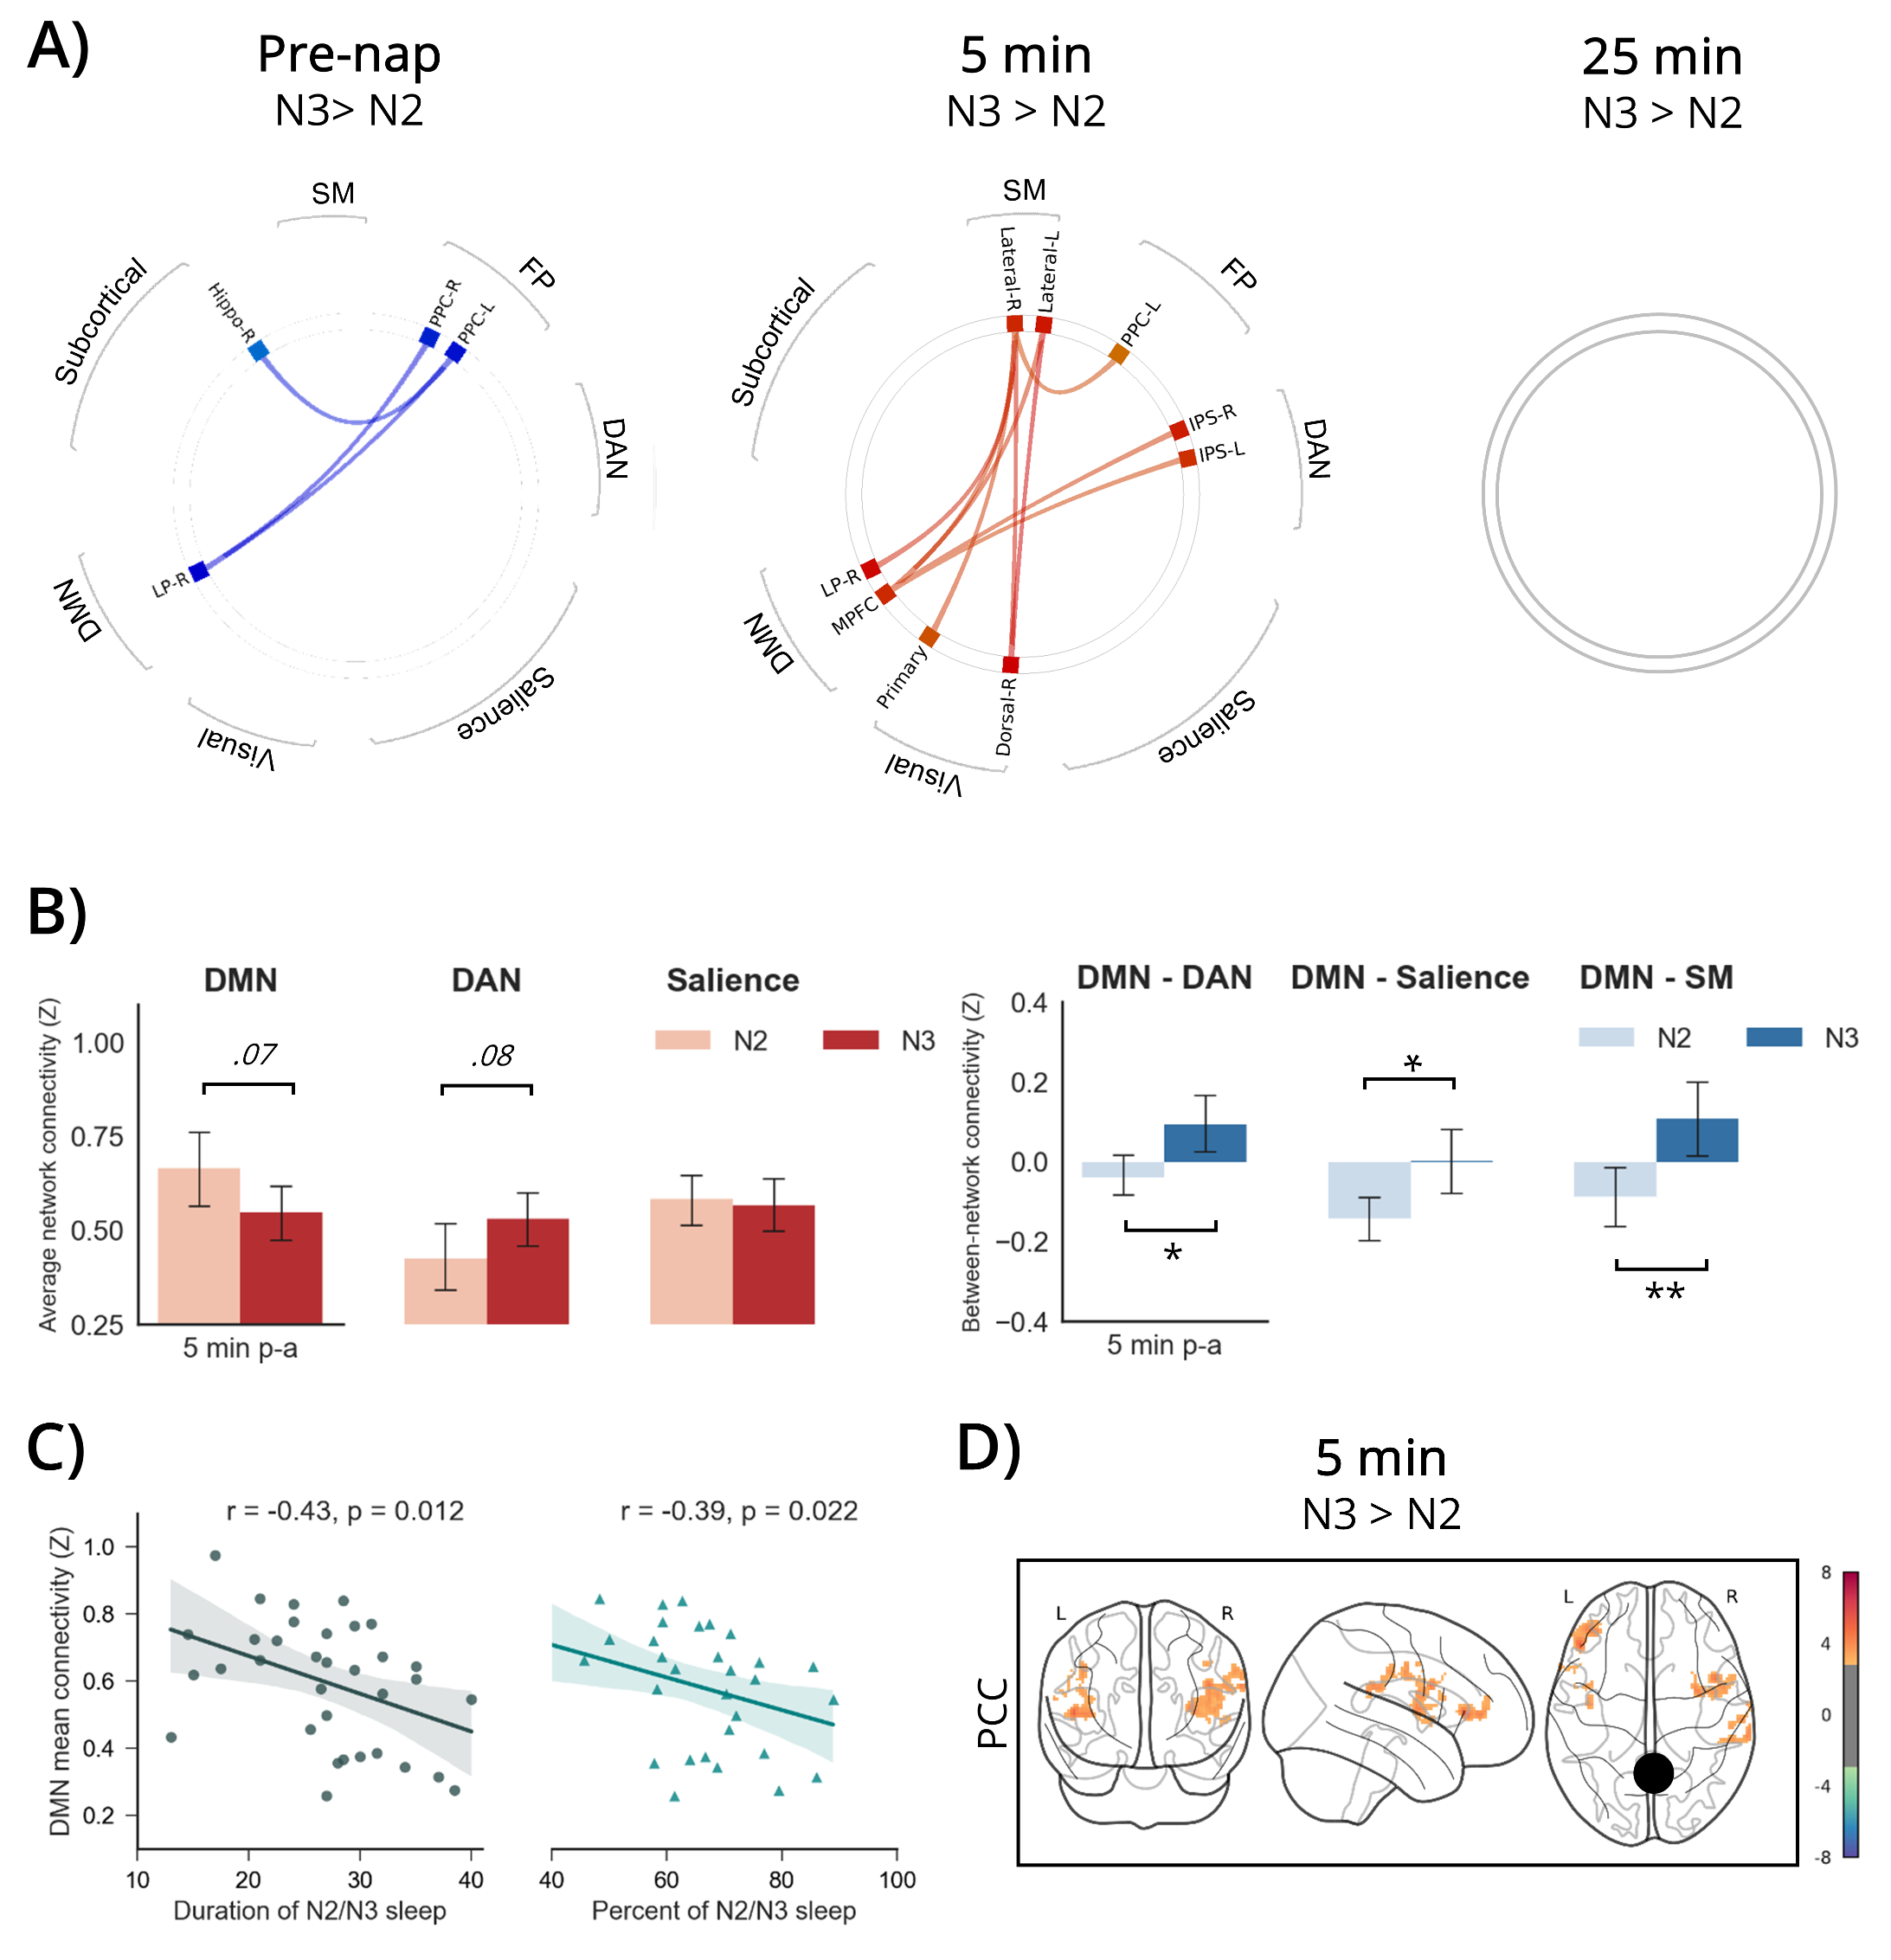
\includegraphics[width=\textwidth]{Fig/Results/Inertia/Inertia/Fig5_N2vsN3.png}
	\caption*{\textbf{Fig 5. Comparison of the functional connectivity after awakening from N3 sleep (n=20) and N2 sleep (n=14).} (A) ROI-to-ROI results at the pre-nap, 5 min and 25 min p-a scans for the contrast N3 minus N2. Blue connections indicate regions with significantly increased (red lines) or decreased (blue lines) connectivity (two-sided t-test, p<.05 FDR-corrected). No difference was found for the 25 min p-a scan. (B) Mean pairwise connectivity within (left, red bars) and between (right, blue bars) networks. Stars denote significant between-group comparisons (t-tests, * p<.05, ** p<.01). (C) Seed-based connectivity results at 5 min p-a for the contrast N3 minus N2. Seed region is the posterior cingulate cortex (PCC), one core region of the DMN which demonstrates notable disruption during NREM sleep (center of mass in MNI coordinates: 1, -61, 38). Statistical parametric maps are reported using an uncorrected two-sided cluster-defining voxel-wise height threshold of p<.01 and a whole-brain FWE-corrected extent threshold of p<.05. Yellow-red colors indicate increased connectivity at pre-nap and/or 25 min p-a compared to the 5 min p-a scan. Green-blue colors indicate increased connectivity at 5 min p-a compared to the two other scans.}
\end{figure}

\FloatBarrier

\subsection*{Discussion}
\label{res:inertia:inertia:discussion}

In a recent review on sleep inertia, \citet{trotti_waking_2016} proposed as first item on a 5-items research agenda that q{if as suggested by PET imaging, resumption of normal waking cognition on awakening requires reorganization of cognitive networks, can other functional neuro-imaging and/or neurophysiologic studies better delineate these necessary network changes?}. The present study aimed at addressing this issue using combined EEG-fMRI, by characterizing the changes in brain networks functional connectivity across the first half hour following awakening from NREM N2 and N3 sleep (resting state scans acquired at 3 time points : pre-sleep, 5 and 25 minutes post-awakening). By contrast with previous studies we also measured behavioral performance (DST) and maximized sleep inertia by partially sleep-depriving the subjects on the night before the experiment, and awakening them after a sustained period of N2 and/or N3 sleep when possible.

\subsubsection*{Performance impairments at awakening}
Using the DST we managed to evidence a decrement in performance after awakening even though the measure was made about 9 minutes after awakening (duration of the resting state scan = 6 min + the average delay between awakening and the scan onset = 3 ± 2 min). We indeed chose to favor the estimation of functional connectivity over the estimation of performance at awakening. For this reason behavioral effects were most probably underestimated in our study.

We found no significant decrement in performance at 5 min p-a compared to pre-sleep. This may be due to the delay between awakening and the first DST and/or to the fact that participants were tired before the nap due to their short night sleep. The total number of responses however was reduced, regardless of the awakening sleep stage and without any significant change in the number of mistakes, at 5 minutes p-a compared to 25 minutes p-a. This observation confirms that sleep inertia effects are conspicuous after a short daytime nap, comprising or not N3 sleep, and is consistent with the generally held view that speed is more impaired than accuracy at awakening \citep{tassi_sleep_2000, trotti_waking_2016}. The relatively smaller decrement in performances observed in the present study compared to previous studies that have used the DST immediately after awakening \citep{dinges_assessing_1985, evans_recovery_1975, stampi_ultrashort_1990} may be accounted for by the delay between the awakening and the task. Our results may therefore suggest that the behavioral aspects of sleep inertia evolve rapidly after awakening and/or are compensated by the beneficial effect of sleep on cognitive performance \citep{faraut_napping:_2016}.

Interestingly we found significantly more mistakes in the N2 group than in the N3 group at 5 min p-a. This finding comes against the idea that the deeper the sleep prior awakening, the worse the performance upon awakening. One explanation could be that the beneficial effect of deep sleep may exceed the detrimental effect of sleep inertia, especially after the above-mentioned 9 min delay between awakening and the first post-sleep DST. Second, this effect may be task-specific. Indeed, the functional connectivity disruptions observed at 5 min p-a from N2 and N3 sleep certainly impact different tasks differently. To our knowledge, no previous studies reported DST performance separately for N2 and N3 sleep. According to our results, the functional connectivity disruptions observed at 5 min p-a from N2 impacts more the performance at the DST than the functional connectivity disruptions observed at 5 min p-a from N3 sleep. The impact on performance may have been reversed if we had used a different task.

\subsubsection*{Functional connectivity alterations after awakening from N3 sleep}
Awakening from N3 sleep was associated with robust and global alterations in the brain connectivity. The most significant finding was the decreased anti-correlation between networks normally anti-correlated during resting wakefulness, such as the task-negative (DMN) on the one hand and the task-positive (DAN, salience) networks on the other hand. This disruption of anti-correlation between task-positive and task-negative networks has been observed in a large palette of states including general anesthesia \citep{boveroux_breakdown_2010}, sleep deprivation \citep{de_havas_sleep_2012, samann_increased_2010, wang_spontaneous_2016} and most importantly during NREM sleep \citep{larson-prior_modulation_2011, samann_development_2011}. This suggests that the functional connectivity during the first minutes following awakening from N3 sleep is marked by an intrusion of sleep specific connectivity into the wakefulness state. Another key finding was that as compared to 5 min p-a, the functional connectivity at 25 min p-a was partially restored between the DMN and DAN and between the thalamus and the frontoparietal network. This change in the dynamic of thalamo-cortical connectivity corroborates previous EEG studies that showed a progressive dissipation of slow wave activity during sleep inertia \citep{ogilvie_falling_1992, ferrara_electroencephalographic_2006, marzano_recalling_2011, gorgoni_eeg_2015}. Finally, using seed-based analyses, we were able to evidence a decreased connectivity between the PCC and the inferior / middle temporal gyrus at 5 min p-a compared to pre-sleep. The middle temporal gyrus has been recently described as part of a DMN subcomponent involved in memory, constructive mental simulations, and according to the author’s postulate, dreaming \citep{christoff_mind-wandering_2016}. It is noteworthy that we observed a reduced connectivity of this region after awakening from N3 sleep which is well known to lead to less dream reports than any other sleep stages \citep{nielsen_review_2000, ruby_experimental_2011}.

\subsubsection*{Functional connectivity alterations after awakening from N2 sleep}
Participants awakened in N2 sleep exhibited little alterations regarding the DMN connectivity and anti-correlations using ROI-to-ROI analysis. One notable exception is the increased connectivity between the DMN and hippocampus at 5 min p-a compared to pre-sleep, which has been reported to predicts subjective sleepiness and worsened working-memory performance under conditions of sleep loss (see \citealp{krause_sleep-deprived_2017}). This and the relative decrease of connectivity in the FP network observed in both ROI-to-ROI and seed-based analysis, could therefore be good candidates to explain the increased percent of mistakes in the N2 group at 5 min p-a compared to the N3 group. Apart from this, we have found at 5 min p-a compared to both pre-sleep and 25 min p-a a strong decrease in the connectivity between the SM and FP networks as well as an increased connectivity between the visual and salience networks. A suboptimal functional connection between the somato-motor network and the executive network may explain the decreased sensori-motor performances (e.g. grip strength, steadiness and coordination) after awakening from N2 sleep reported in several behavioral studies. Similarly the reduced functional connection between the visual and the salience network may be the reason for the deficits in visuo-perceptual tasks at awakening (see \citealp{tassi_sleep_2000}). Finally, at 5 min p-a compared to pre-sleep, seed-based analysis revealed a large increase in the connectivity between the PCC and the parahippocampal gyrus, a region involved in memory retrieval. Such a functional modification may participate in the well-known variability in dream recall between sleep stages \citep{nielsen_review_2000, ruby_experimental_2011}.

\subsubsection*{Link between functional alterations and prior sleep depth / duration}
Several conclusions may be drawn in the light of the above. Awakenings from N2 and N3 sleep were both associated with alterations in functional connectivity. Some of these alterations overlapped and some did not. Regarding the overlap, in both sleep stages we have found strong alterations in the SM network at 5 min p-a. This disruption of SM connectivity was previously reported in two previous studies \citep{wu_variations_2012, tsai_local_2014} and appears to be the physiological signature of the motor impairments and clumsiness classically reported during sleep inertia. Most importantly, there were also several discrepancies in the alterations following N2 or N3 sleep awakening. N3 sleep was characterized by a more robust loss of functional segregation between several networks. Notably, we found large reductions in the anti-correlation between the DMN and task-positive networks (FP, DAN, SM, Salience) as well as an increased connectivity between sensory networks (visual and FP). One key finding is the negative significant correlation between the average DMN mean connectivity and the duration (and percentage) of N2 and N3 sleep during the nap. This result and the previous ones suggest that alterations in the DMN functional connectivity upon awakening are directly linked to the prior sleep duration and depth at least in the first sleep cycle. From a phenomenological standpoint, the intense disruption of the DMN connectivity after awakening from N3 sleep may account for internally-oriented cognitive impairments such as feeling of disorientation, desire to return to sleep and rapid vanishing of short-term memory content (i.e. dreams) frequently observed after awakening from this sleep stage. By contrast, disrupted anti-correlations between the DMN and attentional networks, in addition with reduced FP connectivity, may explain the hypovigilance and reduced cognitive performances which have been consistently reported during sleep inertia. On a more practical level, our findings provide experimental evidences in favor of the general public health advice to take short naps (< 20-30 min) in order to avoid entering N3 sleep, which may suppress the cognitive advantage of taking a nap.

\subsubsection*{Limitations}
Due to the partial sleep deprivation, the functional connectivity during the pre-sleep scan was probably altered as compared to rested wakefulness after a full night of sleep \citep{samann_increased_2010, de_havas_sleep_2012, yeo_functional_2015, kaufmann_brain_2015, tushaus_resisting_2017}. It follows that our results most probably underestimate the functional connectivity disruption associated with sleep inertia. Finally, it is also possible that the MRI scan noise may have had a positive alerting effect on vigilance and therefore reduced the severity of sleep inertia. However, only one study has so far investigated the effect of a pink noise at 75 dB on sleep inertia. The authors reported inconclusive results on whether noise improved or worsened sleep inertia effects after a nap \citep{tassi_effects_1992}.

\subsubsection*{Conclusion}
The present combined EEG-fMRI study provides for the first time a measure of both brain functional connectivity and behavioral performance at 5 and 25 minutes post awakening from N2 and N3 NREM sleep. By splitting participants who were awakened in N2 and N3 sleep, and thanks to a large number of participants (n=55), we were able to provide an exhaustive overview of the functional connectivity alterations following awakening from these two sleep stages. Our results support the hypothesis of \citet{balkin_process_2002} and show that the functional connectivity is altered at awakening from both N2 and N3 sleep, but in a much severe way after an awakening from N3 sleep. Importantly, awakening from N3 sleep induced a severe disruption of the functional connectivity in the default mode network which was not the case for awakening from N2 sleep. In addition, awakenings from N3 sleep were associated with a robust loss of brain functional networks segregation, which severity was correlated with prior sleep duration. Our result provide, as whished by \citet{trotti_waking_2016} in her recent review, the q{which an how} functional brain networks are altered at awakening and show that sleep inertia is the result of an intrusion of sleep specific features in the functional connectivity of the awake brain.

\paragraph{Acknowledgments}
The authors would like to thank Basak Turker, Morgane Hamon, Franck Lamberton and Danielle Ibarrola for substantial help in data collection and analysis, as well as Jamila Lagha for her help in administrative work.

\paragraph{Author contribution}
R.V and P.R designed the study, acquired the data and wrote the paper. D.M helped in data analysis. A.N participated to the design and provided access to his sleep unit to conduct the sleep deprivation.

\newpage

\subsection*{Supplementary materials}
\label{res:inertia:inertia:supp}
\vspace*{1cm}

\begin{figure}[!htbp]
	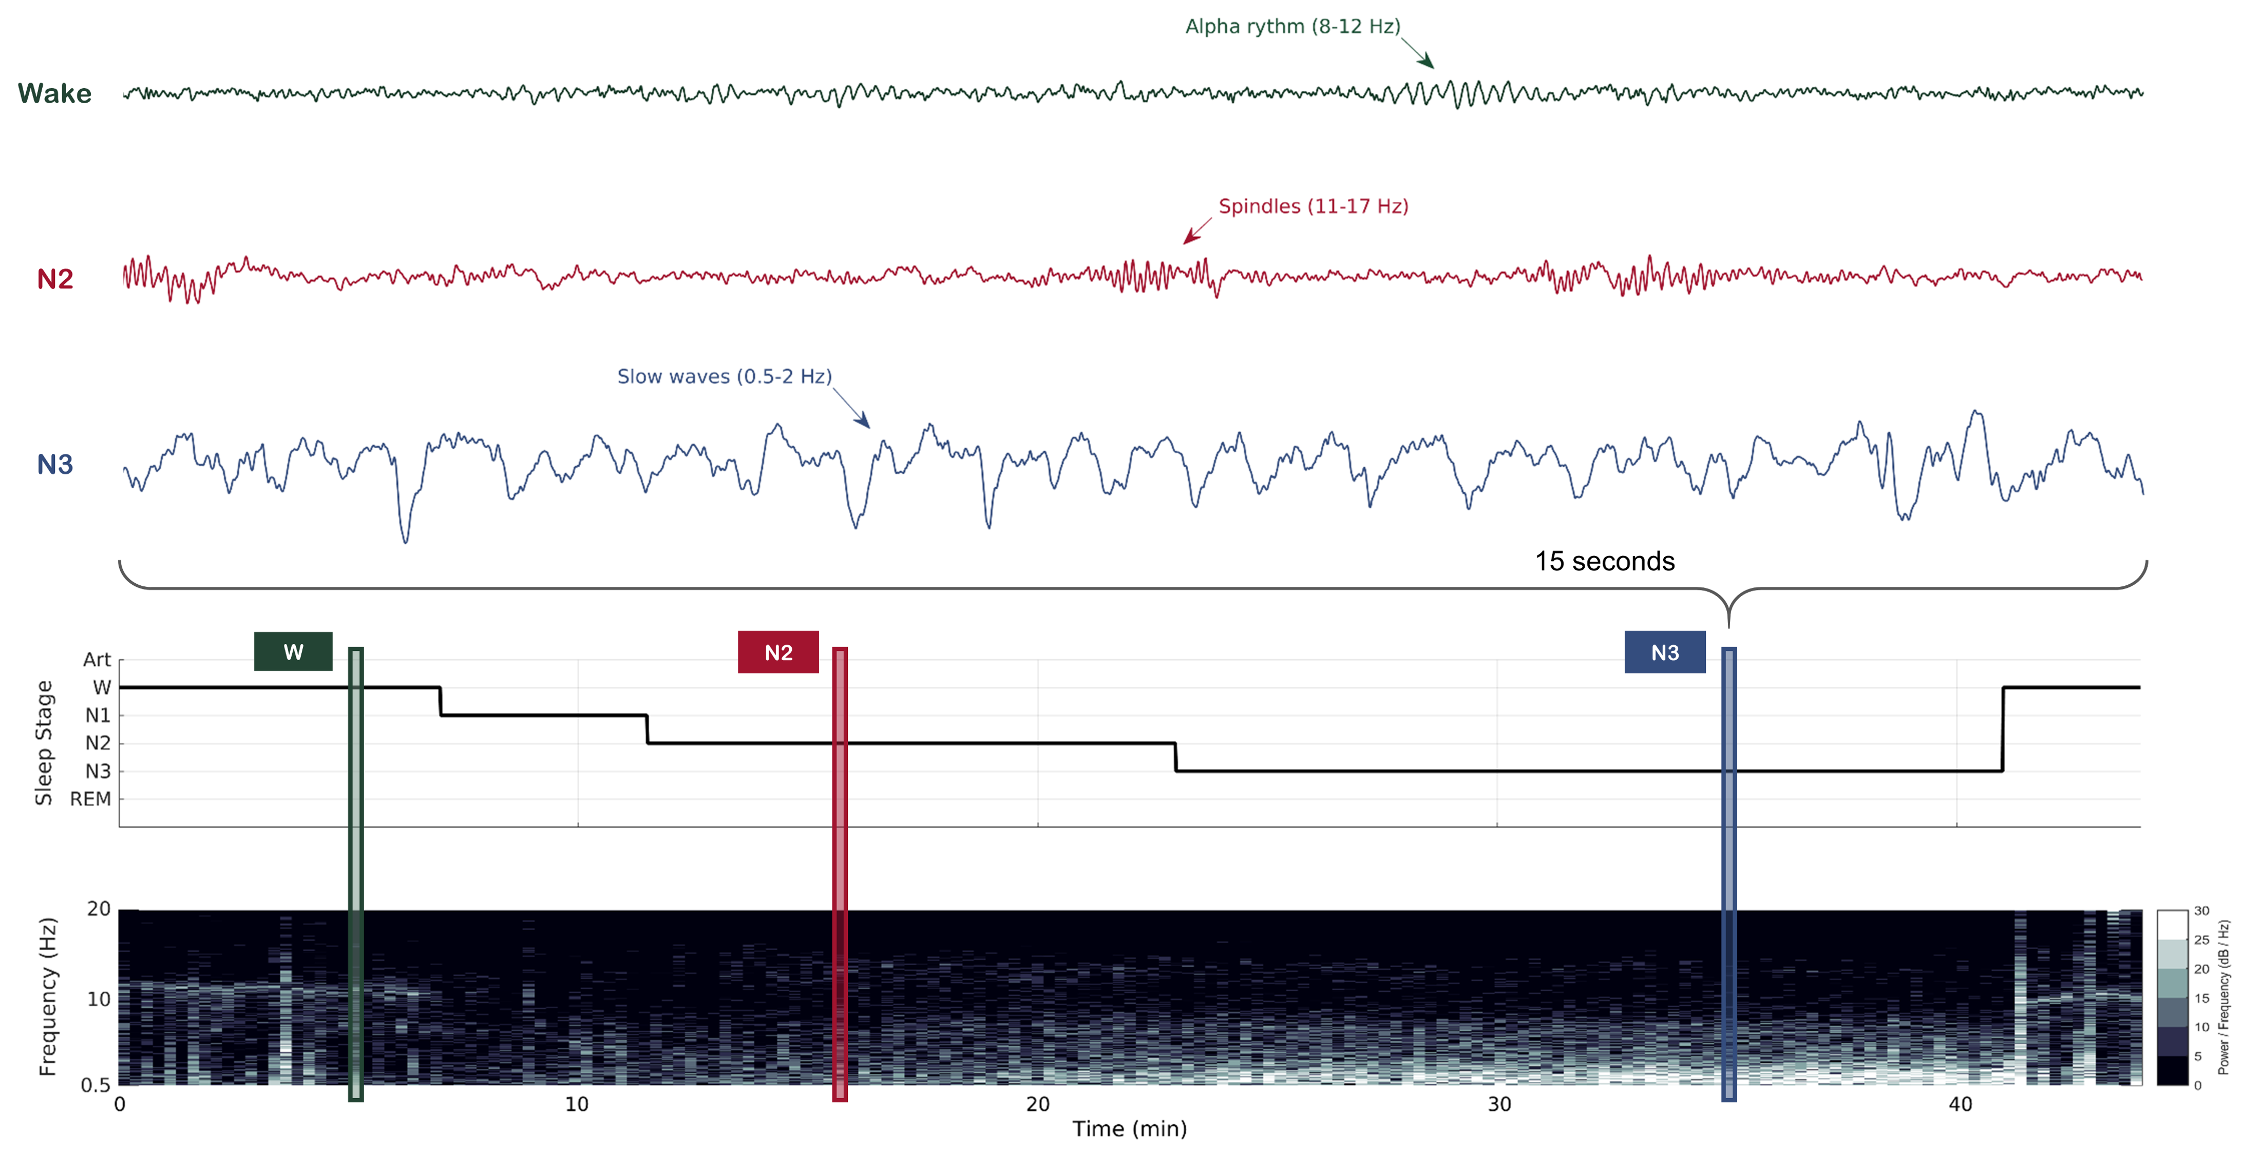
\includegraphics[width=\textwidth]{Fig/Results/Inertia/Inertia/S1_Scoring.png}
	\caption*{\textbf{S1 Fig. Hypnogram and EEG data (Cz) acquired during the nap slot in one subject.} Top. 15-seconds frames of wakefulness, N2 and N3 sleep. Middle. Hypnogram showing vigilance states as function of time during the nap slot. Bottom. Spectrogram showing the normalized power in the 0.5 – 20 Hz range for each 15-seconds frames (lighter colors indicate higher power).}
\end{figure}

\begin{figure}[!htbp]
	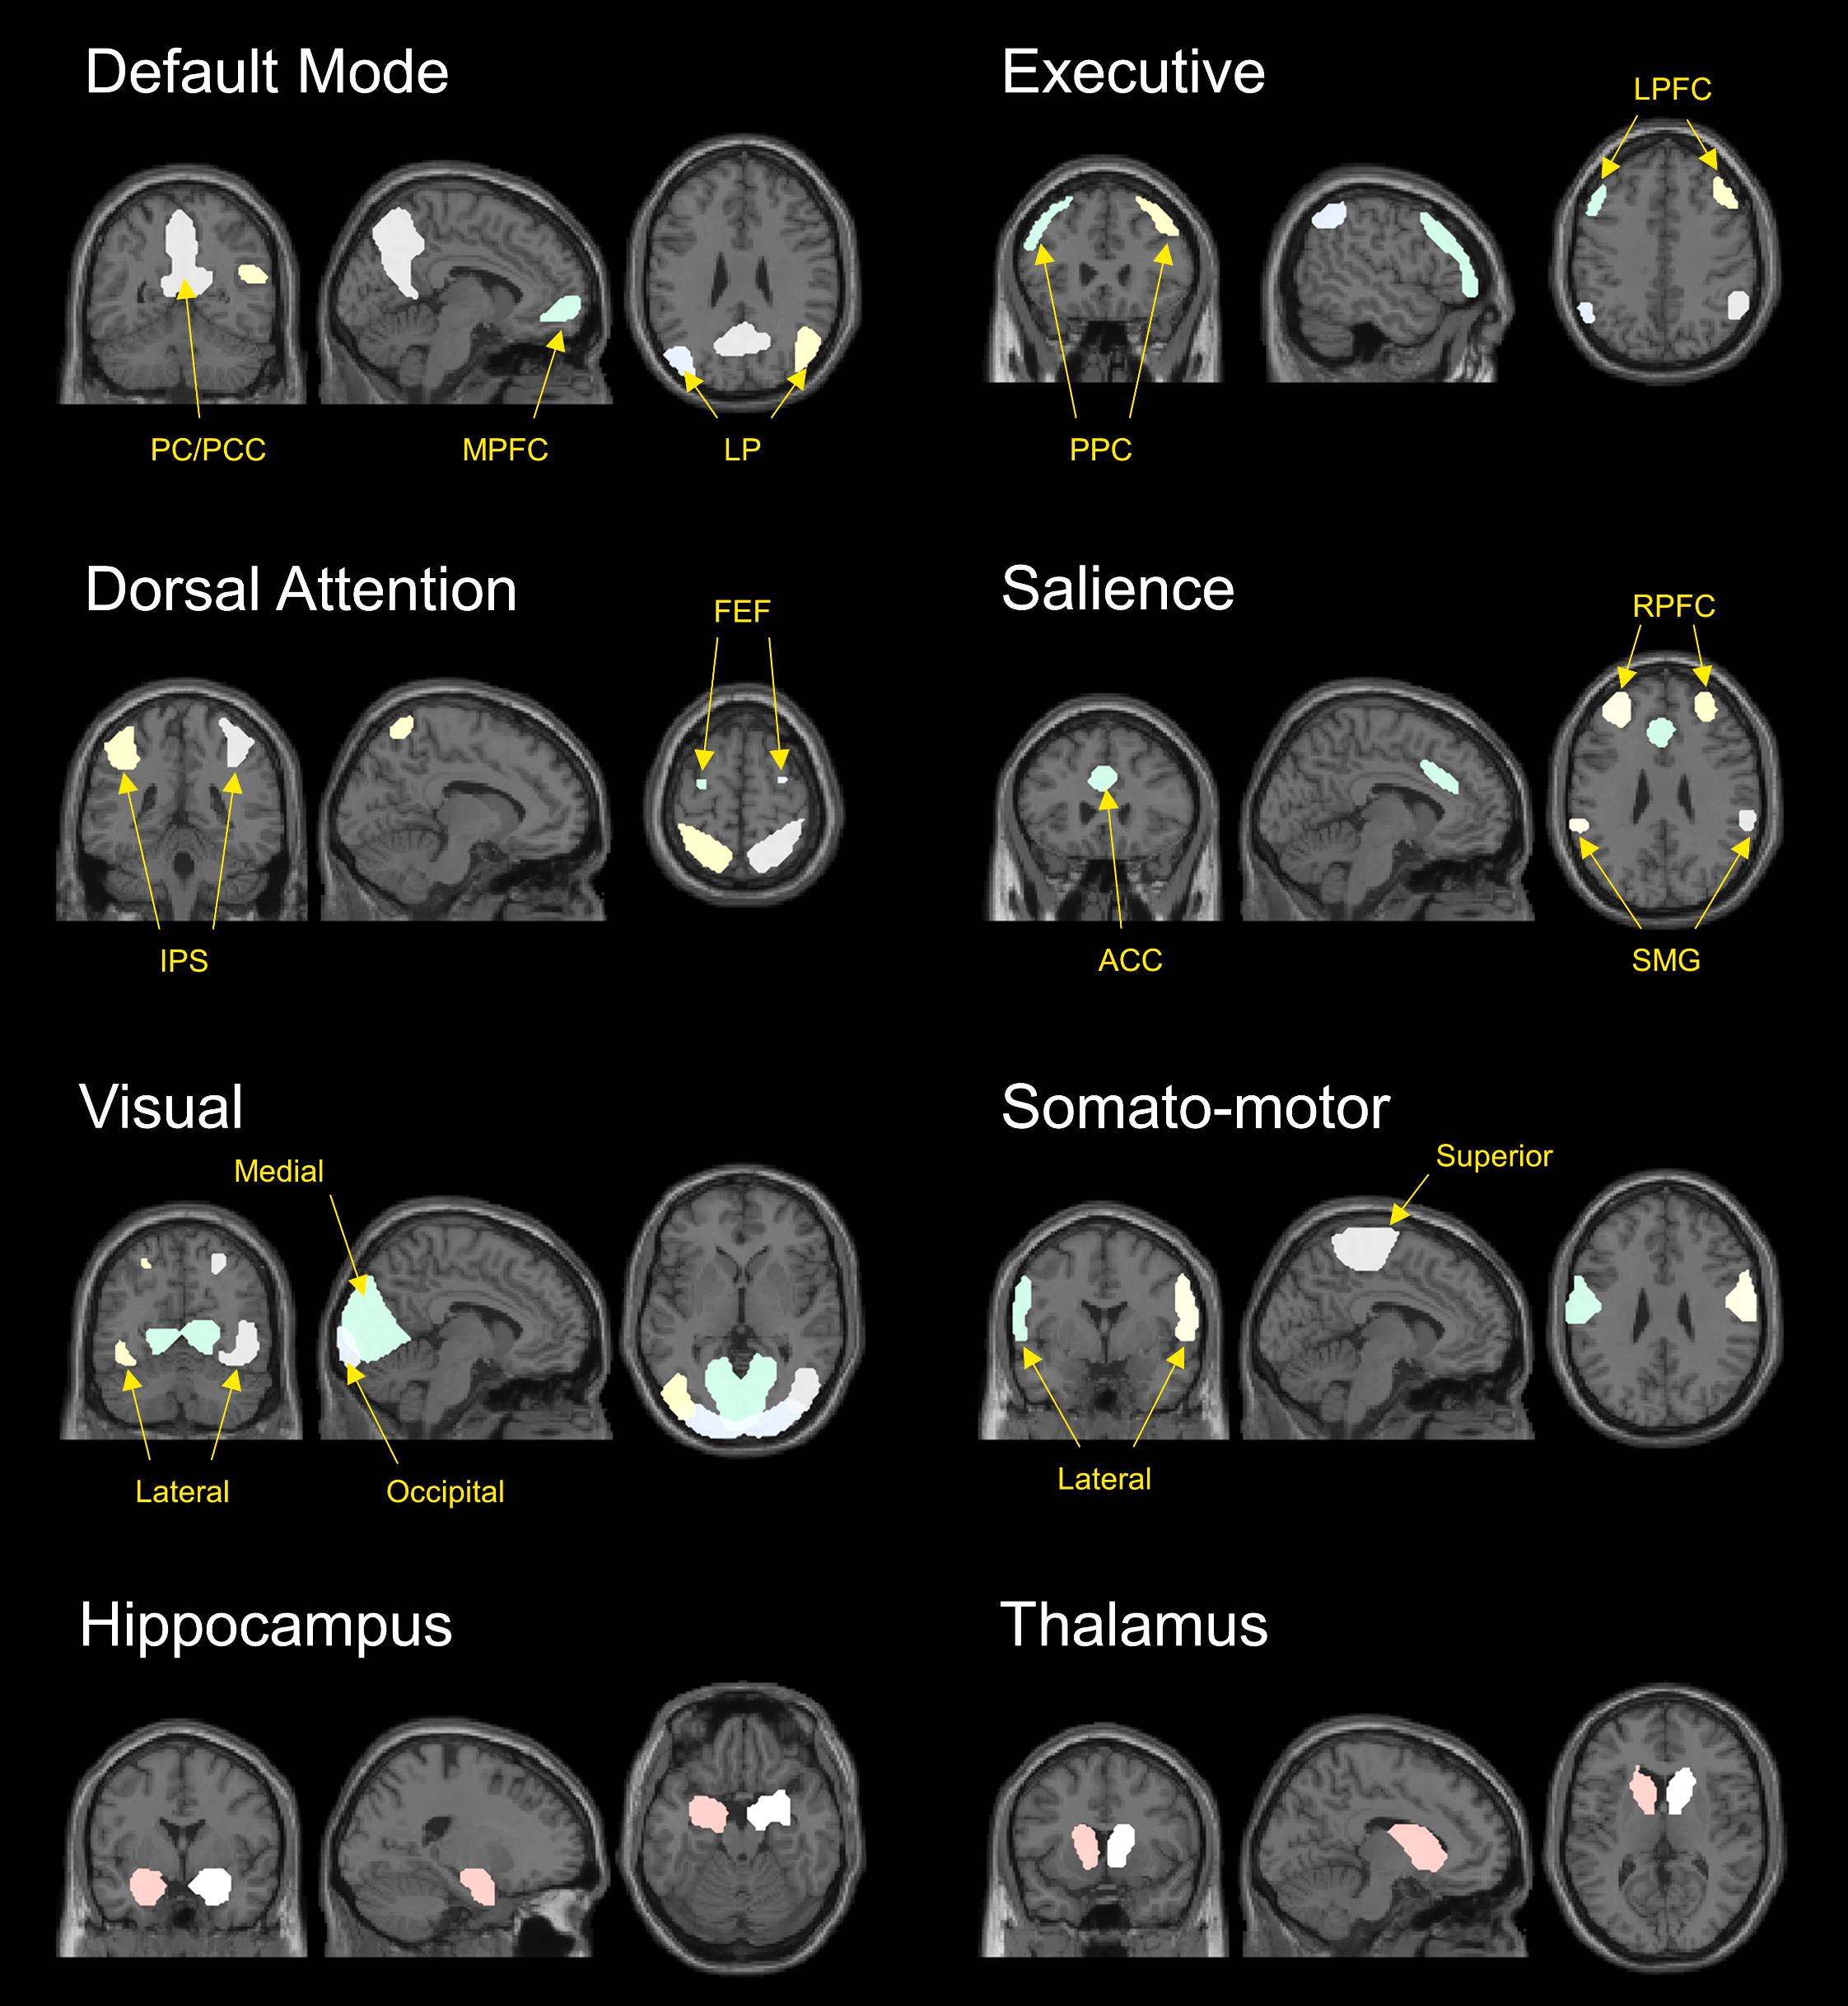
\includegraphics[width=\textwidth]{Fig/Results/Inertia/Inertia/S2_Networks.png}
	\caption*{\textbf{S2 Fig. Networks and regions included in the connectivity analysis.} Abbreviations: PCC/PC, Posterior Cingulate Cortex / Precuneous – MPFC, Medial Prefrontal Cortex – LP, Lateral Parietal – FEF, Frontal Eye Fields – IPS, Intraparietal Sulcus – PPC, Posterior Parietal Cortex – LPFC, Lateral Prefrontal Cortex – ACC, Anterior Cingulate Cortex – RPFC, Rostral Prefrontal Cortex – SMG, Supra-Marginal Gyrus. Note that the salience network also includes the anterior insula (not visible).}
\end{figure}

\FloatBarrier

% Table column width
\newcolumntype{b}{>{\hsize=0.2\textwidth}X}

\begin{table}[htb]
    \caption*{\textbf{S1 Table. Seed-based functional connectivity results for the N3 group (n=20)}. Seed region is the posterior cingulate cortex (PCC, center of mass in MNI coordinates = 1, -61, 38). Statistical analyses were performed using a cluster-defining voxel-wise height threshold of p<.01 (uncorrected, two-sided) and a whole-brain family-wise error (FWE) corrected extent threshold of p<.05 to show brain areas either positively or negatively correlated with the seed region. PG, precentral gyrus - SMG, supramarginal gyrus – ITG, inferior temporal gyrus – SPL, superior parietal lobule – SFG, superior frontal gyrus – N.S, not significant.}
    \resizebox{\textwidth}{!}{%
    \begin{tabularx}{\textwidth}{lXXllllX}
    \toprule
             &              &                    	& \multicolumn{3}{c}{MNI coordinates} 	&         	   &              \\
    Contrast                & Region       			& Brodmann area & X   & Y   & Z   		& T value 	   & Cluster size \\ \midrule
    Pre-sleep > 5 min       & PG L 					& BA44          & -42 & 4   & 26  		& -6.45        & 2980         \\
                            & PG R 					& BA6           & 22  & -14 & 58  		& -6.36        & 1462         \\
                            & SMG L              	& BA40          & -34 & -44 & 34  		& -5.05        & 922          \\
                            & ITG L              	& BA20          & -48 & -6  & -36 		& 6.89         & 742          \\
                            & SPL R              	& BA2           & 40  & -38 & 52  		& -5.10        & 390          \\
                            & PG R 					& BA4           & 8   & -26 & 60  		& -4.14        & 295          \\
                            & SFG R              	& BA6           & 10  & 4   & 66  		& -5.51        & 277          \\
    Pre-sleep > 25 min      & N.S 					& -             & -   & -   & -   		& -            & -            \\
    25 min > 5 min          & PG L 					& BA44          & -42 & 4   & 24  		& -6.68        & 1595         \\
                            & SMG L              	& BA40          & -52 & -46 & 44  		& -5.56        & 879          \\ \bottomrule
    \end{tabularx}%
    }
\end{table}

\begin{table}[htbp]
    \caption*{\textbf{S2 Table. Seed-based functional connectivity results for the N2 group (n=14).} Seed region is the posterior cingulate cortex (PCC, center of mass in MNI coordinates = 1, -61, 38). Statistical analyses were performed using a cluster-defining voxel-wise height threshold of p<.01 (uncorrected, two-sided) and a whole-brain family-wise error (FWE) corrected extent threshold of p<.05. DLPFC, dorsolateral prefrontal cortex – PHG, parahippocampal gyrus – SFG, superior frontal gyrus - N.S, not significant.}
    \begin{tabularx}{\textwidth}{lXXllllX}
    \toprule
    &                       &                       & \multicolumn{3}{c}{MNI coordinates}                &              &               \\
    Contrast                & Region          		& Brodmann area & X          & Y         & Z         & T value 		& Cluster size  \\ \midrule
    Pre-sleep > 5 min       & DLPFC R               & BA9/46        & 28         & 40        & 32        & -5.89        & 464           \\
                            & SFG L                 & BA6           & -22        & -2        & 68        & -6.10        & 351           \\
                            & SFG R                 & BA6           & 26         & 2         & 72        & -6.20        & 271           \\
                            & PHG. R    			& BA34          & 22         & -30       & -12       & -8.40        & 258           \\
                            & DLPFC R               & BA9/46        & -38        & 42        & 40        & -7.01        & 254           \\
    Pre-sleep > 25 min      & N.S    				& -             & -          & -         & -         & -            & -             \\
    25 min > 5 min          & N.S    				& -             & -          & -         & -         & -            & -             \\ \bottomrule
    \end{tabularx}%
\end{table}

\begin{table}[htbp]
    \caption*{\textbf{S3 Table. Seed-based functional connectivity results for the group comparison (N3 (n=20) minus N2 (n=14)).} Seed-based functional connectivity results for the group comparison (N3 (n=20) minus N2 (n=14)). Seed region is the posterior cingulate cortex (PCC, center of mass in MNI coordinates = 1, -61, 38). Statistical analyses were performed using a cluster-defining voxel-wise height threshold of p<.01 (uncorrected, two-sided) and a whole-brain family-wise error (FWE) corrected extent threshold of p<.05 to show brain areas either positively or negatively correlated with the seed region. PG, precentral gyrus - IFG, inferior frontal gyrus – SMG, supramarginal gyrus - N.S, not significant.}
    \begin{tabularx}{\textwidth}{lXXllllX}
    \toprule
    &         &                 & \multicolumn{3}{c}{MNI coordinates}                 &              &              \\
    Scan      & Region    		& Brodmann area & X          & Y          & Z         & T value 		& Cluster size \\ \midrule
    Pre-sleep & N.S 			& -             & -          & -          & -         & -            & -            \\
    5 min     & PG R 			& BA44          & 46         & 8          & 26        & 4.63         & 595          \\
              & IFG L           & BA45          & -48        & 32         & 6         & 5.08         & 314          \\
              & PG L 			& BA4           & -42        & -10        & 36        & 4.90         & 264          \\
              & SMG R           & BA40          & 68         & -32        & 26        & 4.46         & 253          \\
    25 min    & N.S & -         & -          & -          & -         & -            & -            \\ \toprule
    \end{tabularx}%
\end{table}
